\section{Tujuan}
\begin{itemize}[label=$\bullet$, itemsep=-1pt, leftmargin=*]
%    \setlength\itemsep{0.5em}
	% \item Students are able to create projects on an IDE
	% \item Students can demonstrate his/her knowledge of the structure of a C program
	% \item Students can demonstrate his/her knowledge of C data types
	% \item Students can demonstrate his/her knowledge of C operators
    % \item Students are able to use function to read inputs from keyboard
    % \item Students are able to use function to print texts on screen
	\item Mahasiswa dapat membuat proyek di dalam IDE
	\item Mahasiswa dapat menunjukkan pengetahuan mereka tentang struktur program dalam bahasa C
	\item Mahasiswa dapat menunjukkan pengetahuan mereka tentang tipe data dalam bahasa C
	\item Mahasiswa dapat menunjukkan pengetahuan mereka tentang operator dalam bahasa C
    \item Mahasiswa mampu menggunakan fungsi untuk membaca masukan dari keyboard
    \item Mahasiswa mampu menggunakan fungsi untuk mencetak teks di layar

\end{itemize}
\section{Mengenal Bahasa C}

Bahasa C dikembangkan oleh Dennis M. Ritchie dan Brian W. Kernighan pada awal tahun 1970.\\
Terdapat beberapa standar untuk bahasa C, standar di sini dapat diartikan sebagai guideline dalam menuliskan bahasa C. Beberapa Standar yang ada:
\begin{enumerate}
	\item  Definisi Kernighan \& Ritchie (K\&R)
    \item ANSI-C (X-3.159 -1989-)
    \item Definisi AT\&T (untuk superset C, C++), dan
    \item GNU Coding Standards.
\end{enumerate}
\subsection*{}Aplikasi atau kegunaan Bahasa C
\begin{enumerate}
	\item     Membuat sistem operasi dan program-program sistem.
    \item Pemrograman yang "dekat" ke perangkat keras (misalnya untuk kontrol peralatan).
    \item Membuat tool kit.
    \item Menulis program aplikasi.
\end{enumerate}
\section{IDE (Integrated Development Environment)}
IDE adalah singkatan dari "Integrated Development Environment" dalam bahasa Inggris. 
Dalam Bahasa Indonesia, IDE dapat diterjemahkan menjadi "Lingkungan Pengembangan Terintegrasi" atau "Ruang Kerja Pengembangan Terpadu." 
IDE adalah sebuah perangkat lunak yang dirancang untuk membantu pengembang perangkat lunak dalam proses pengembangan, pengkodean, dan pengujian aplikasi komputer.
\\ 
Berikut ini adalah daftar aplikasi IDE bahasa C yang dapat digunakan.
\begin{itemize}
	\item CodeBlocks
	\item DevC++
\end{itemize}
\section{Membuat proyek baru pada IDE Code::Blocks} 
\subsection{Langkah untuk membuat proyek baru}
\begin{enumerate}
\item Go to File $>$ New $>$ Project 
	\begin{figure}[H]
		\centering
		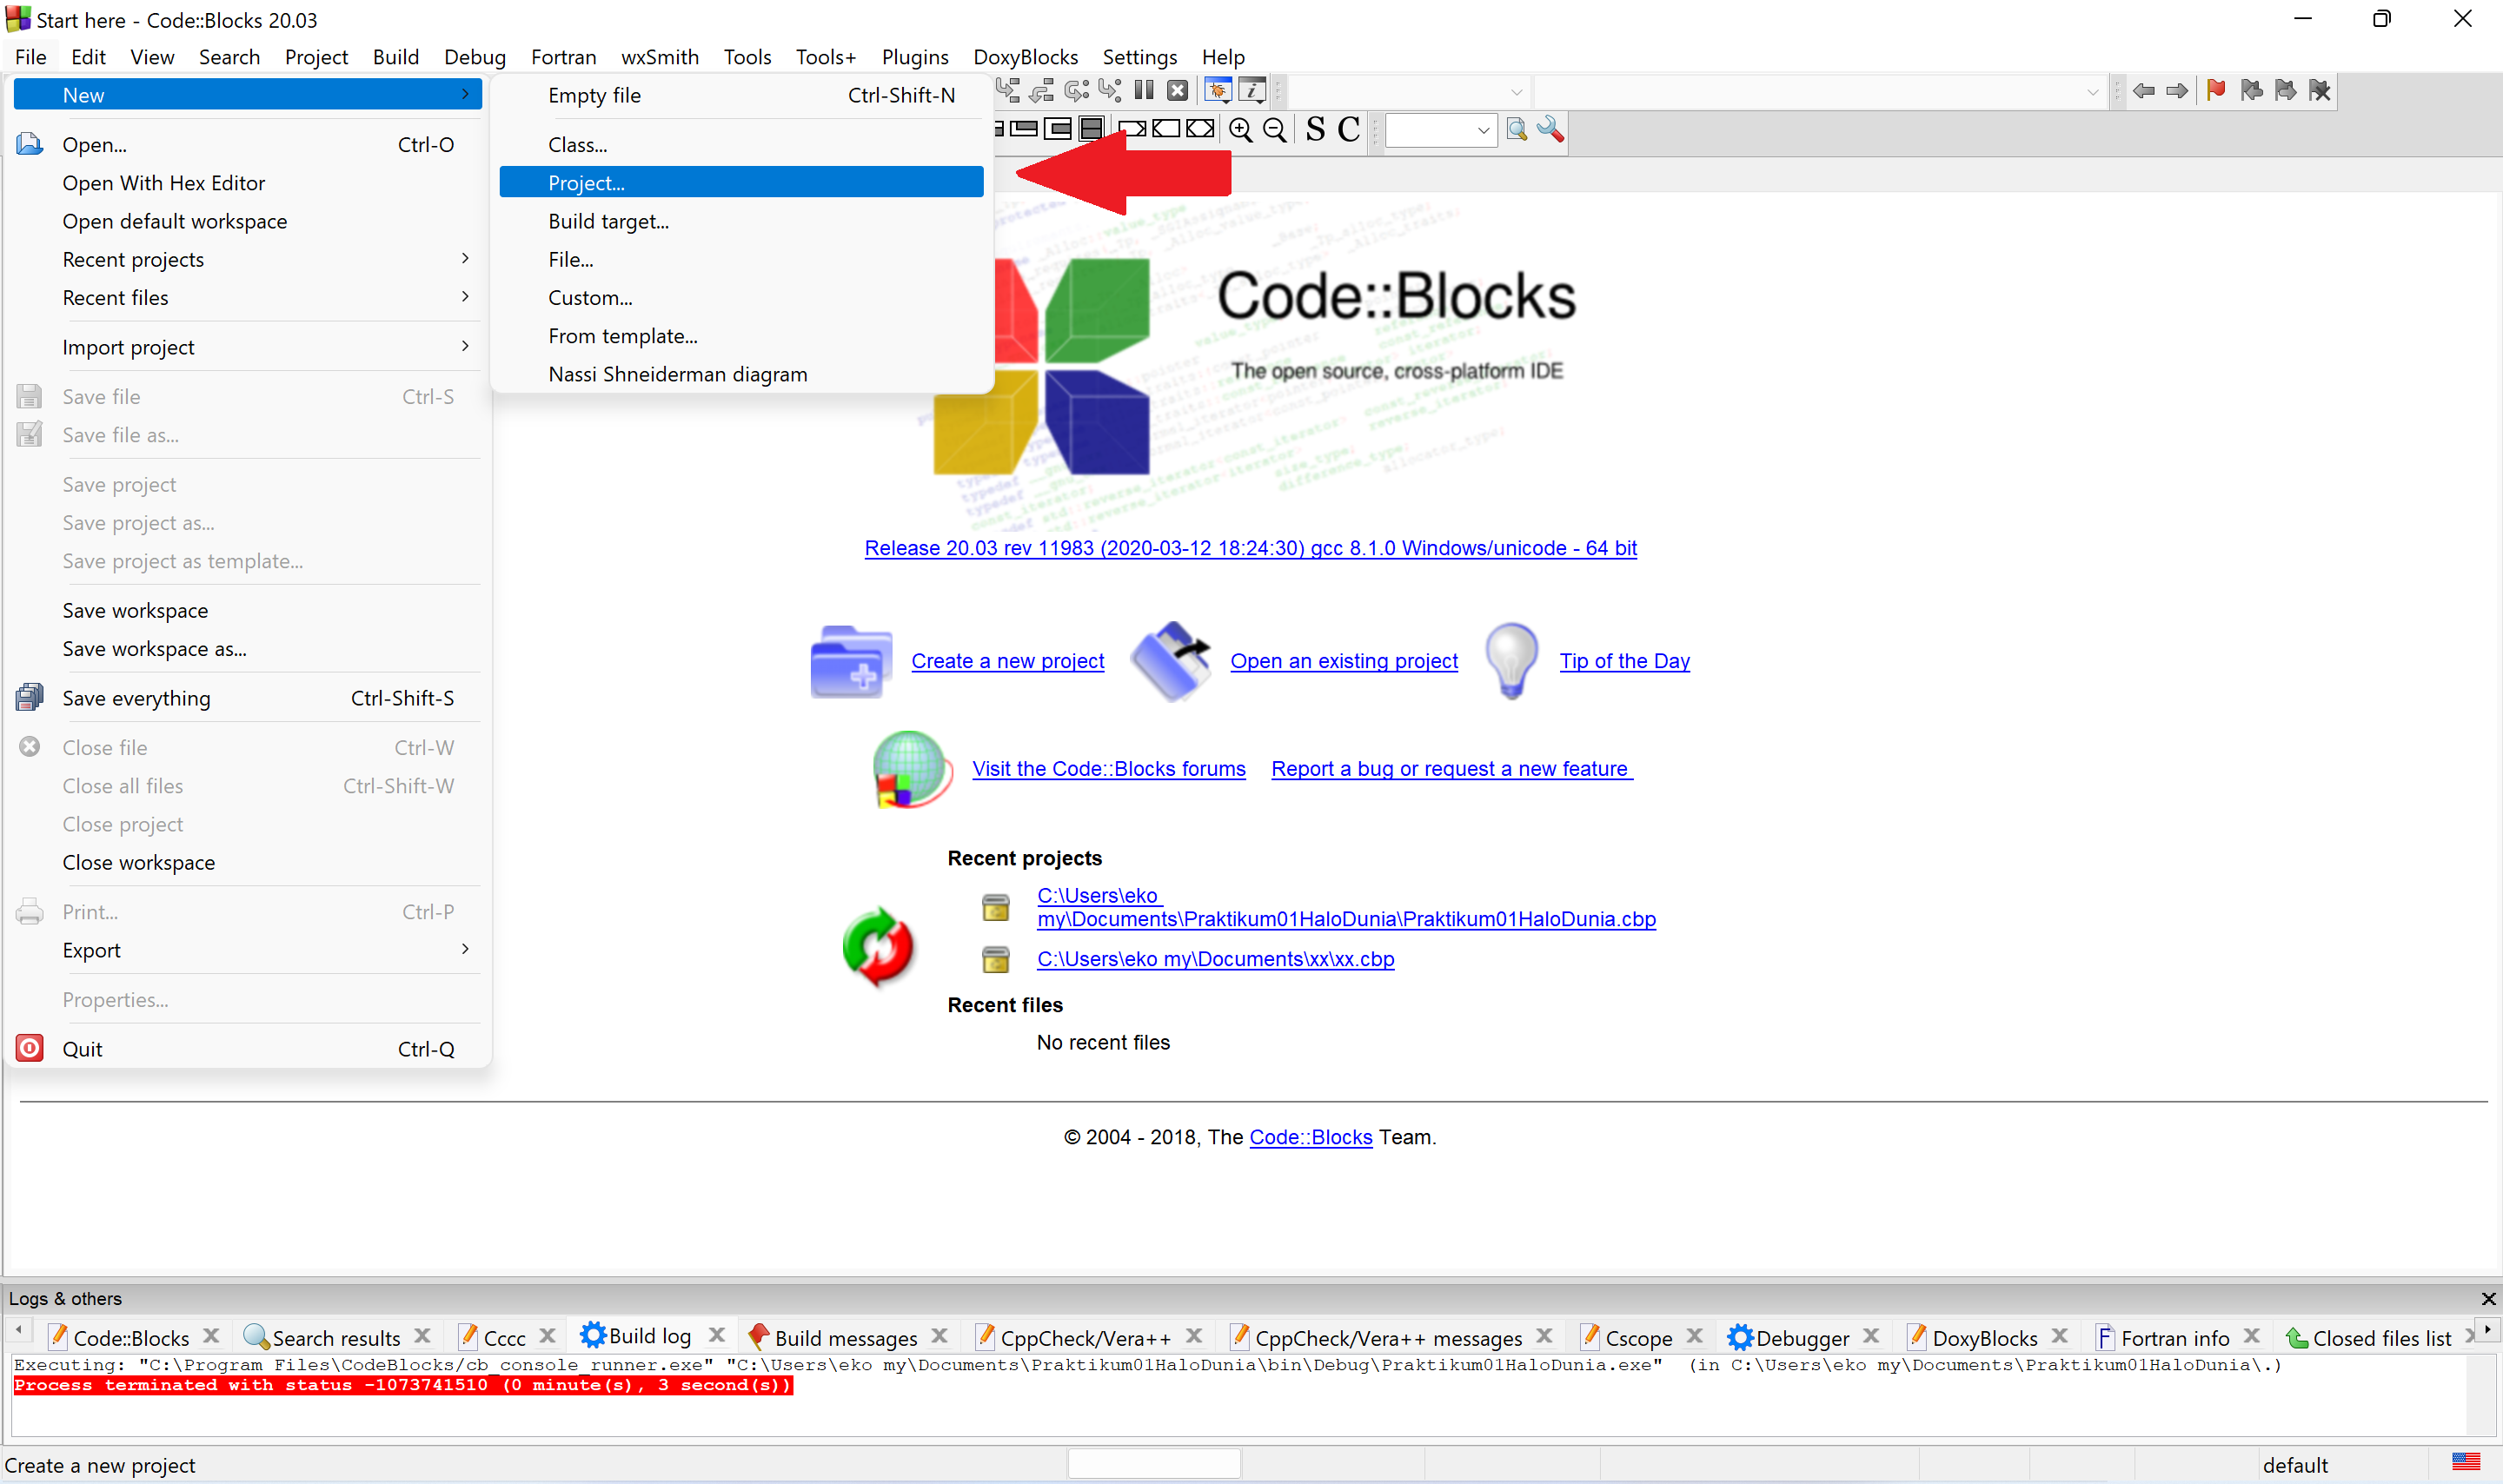
\includegraphics[width=0.7\linewidth]{../P1/img/screenshot002.png}
		\caption{}
		\label{fig:screenshot002}
	\end{figure}
\item Klik Console Application
\begin{figure}[H]
	\centering
	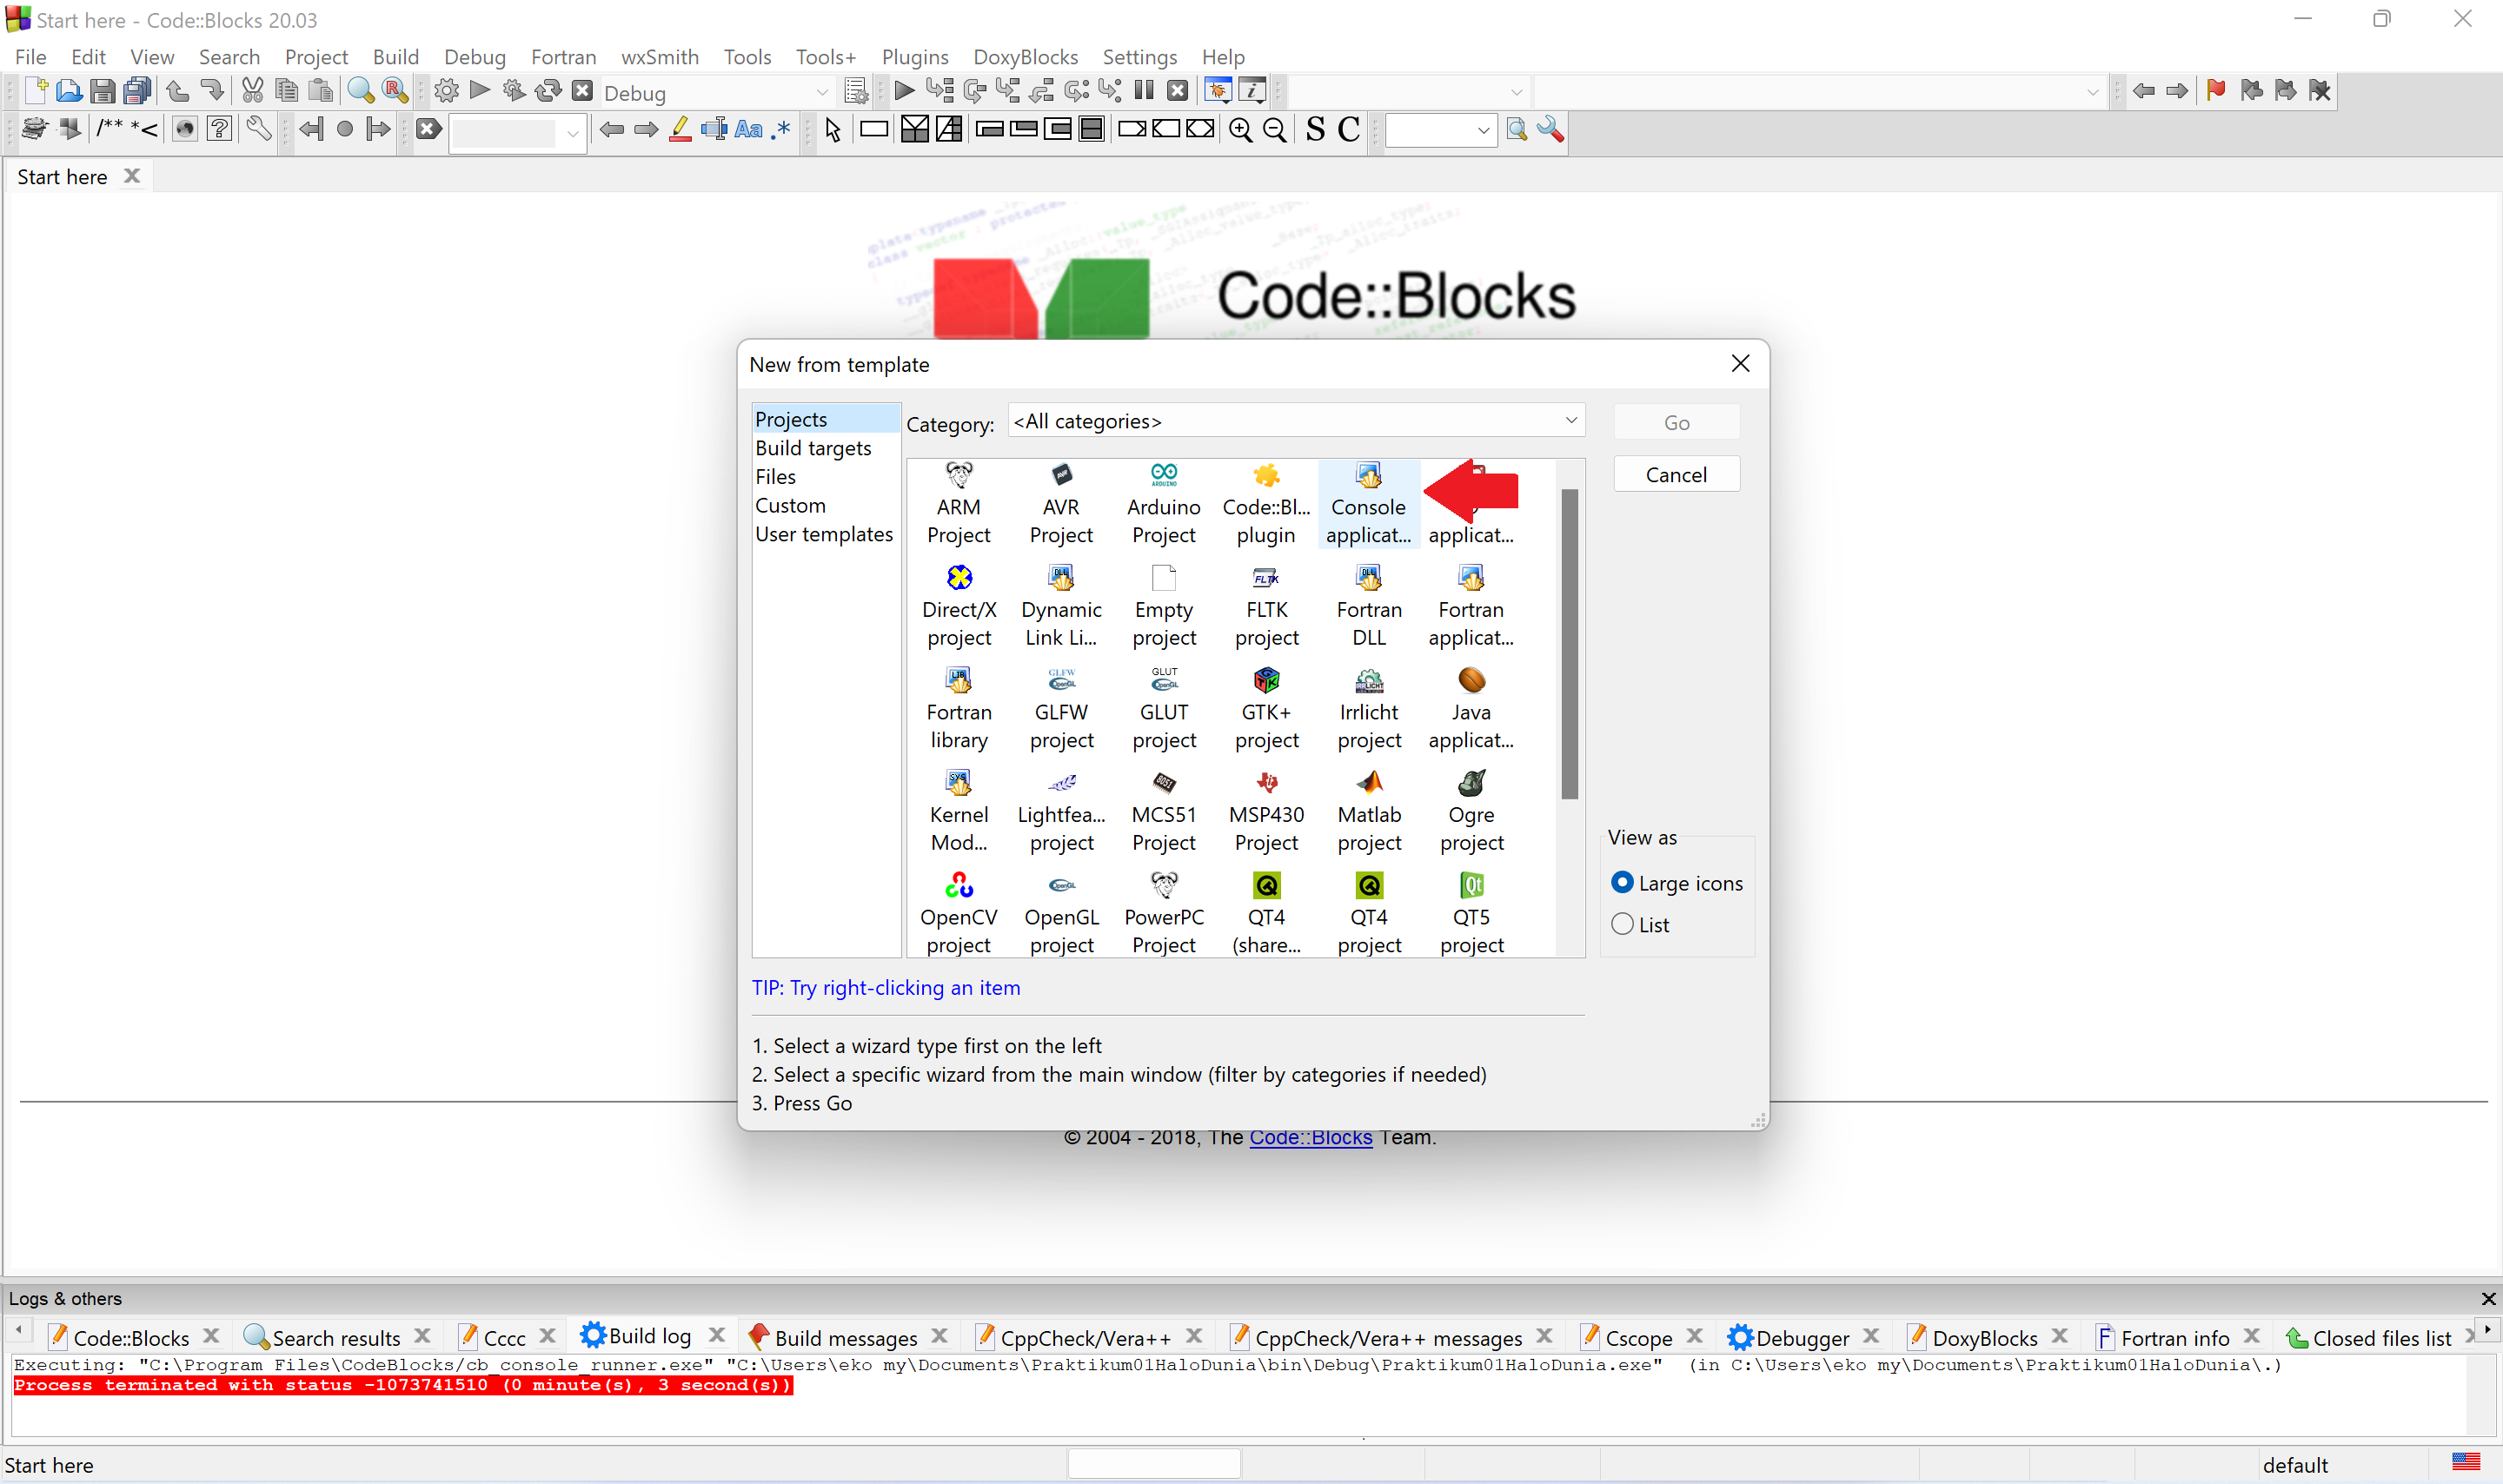
\includegraphics[width=0.7\linewidth]{../P1/img/screenshot004.png}
	\caption{}
	\label{fig:screenshot004}
\end{figure}
\item Pilih C sebagai bahasa Pemrograman
\begin{figure}[H]
	\centering
	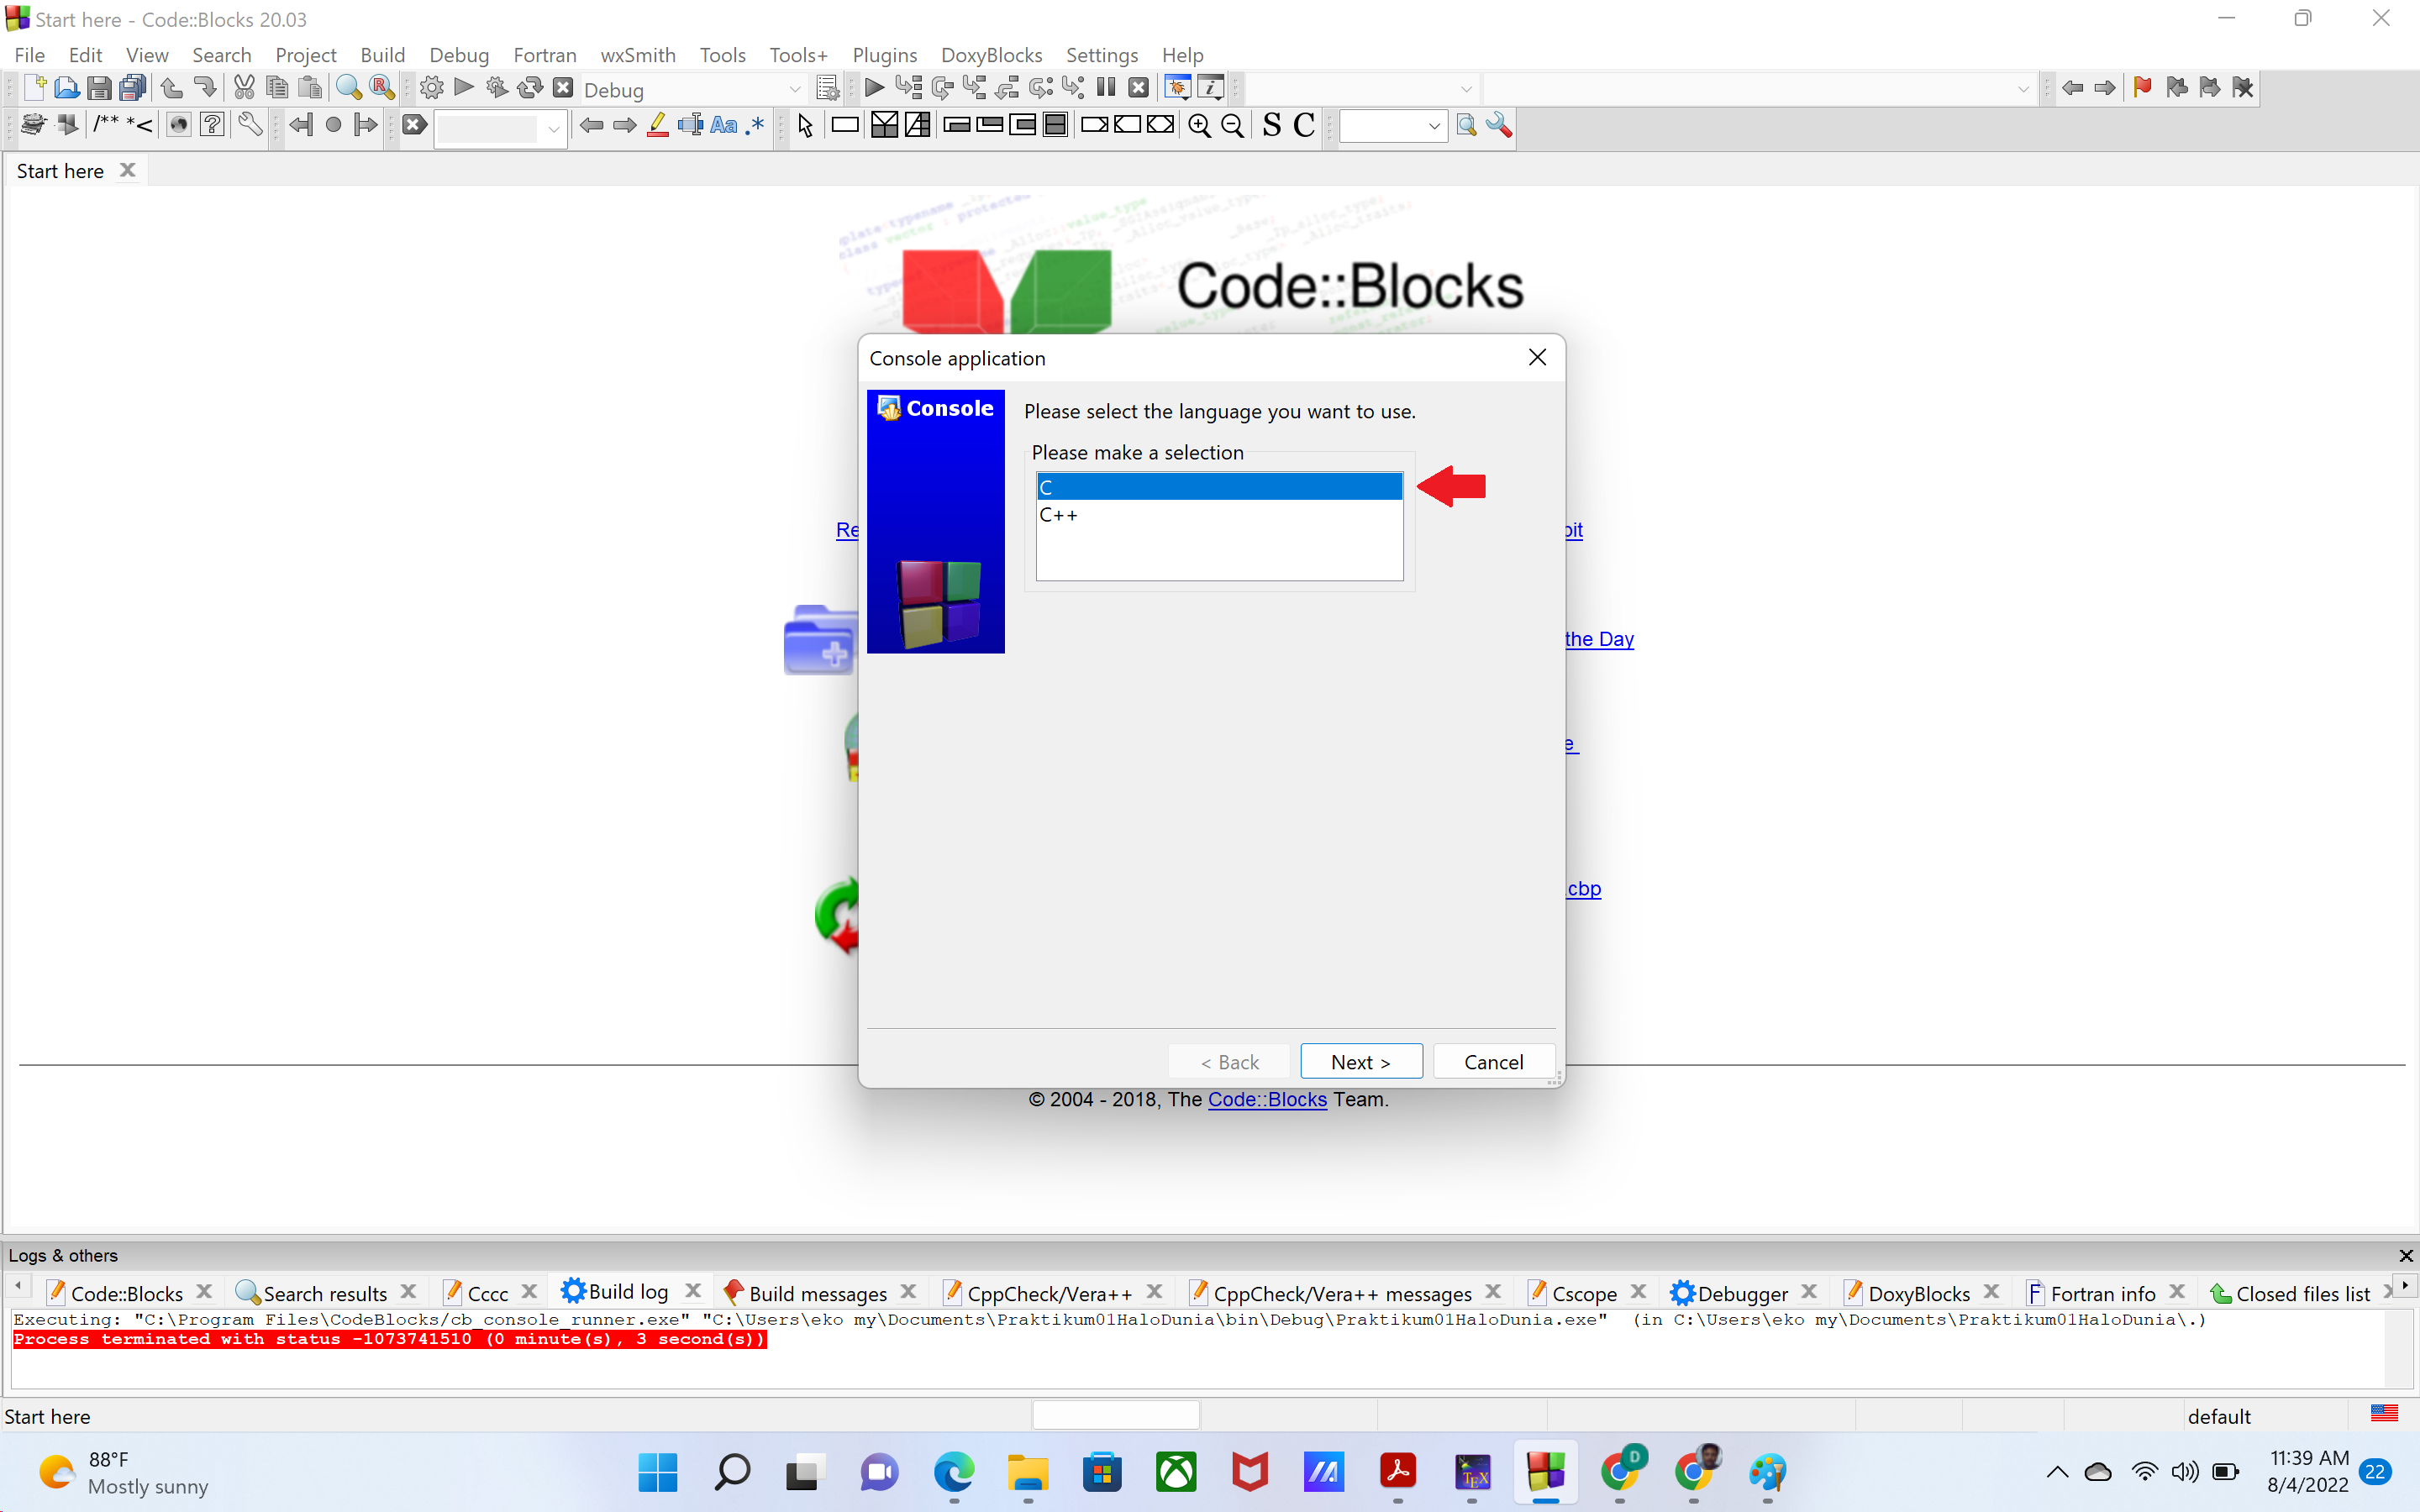
\includegraphics[width=0.7\linewidth]{../P1/img/screenshot005.png}
	\caption{}
	\label{fig:screenshot005}
\end{figure}
\item Berikan nama ke project
\begin{figure}[H]
	\centering
	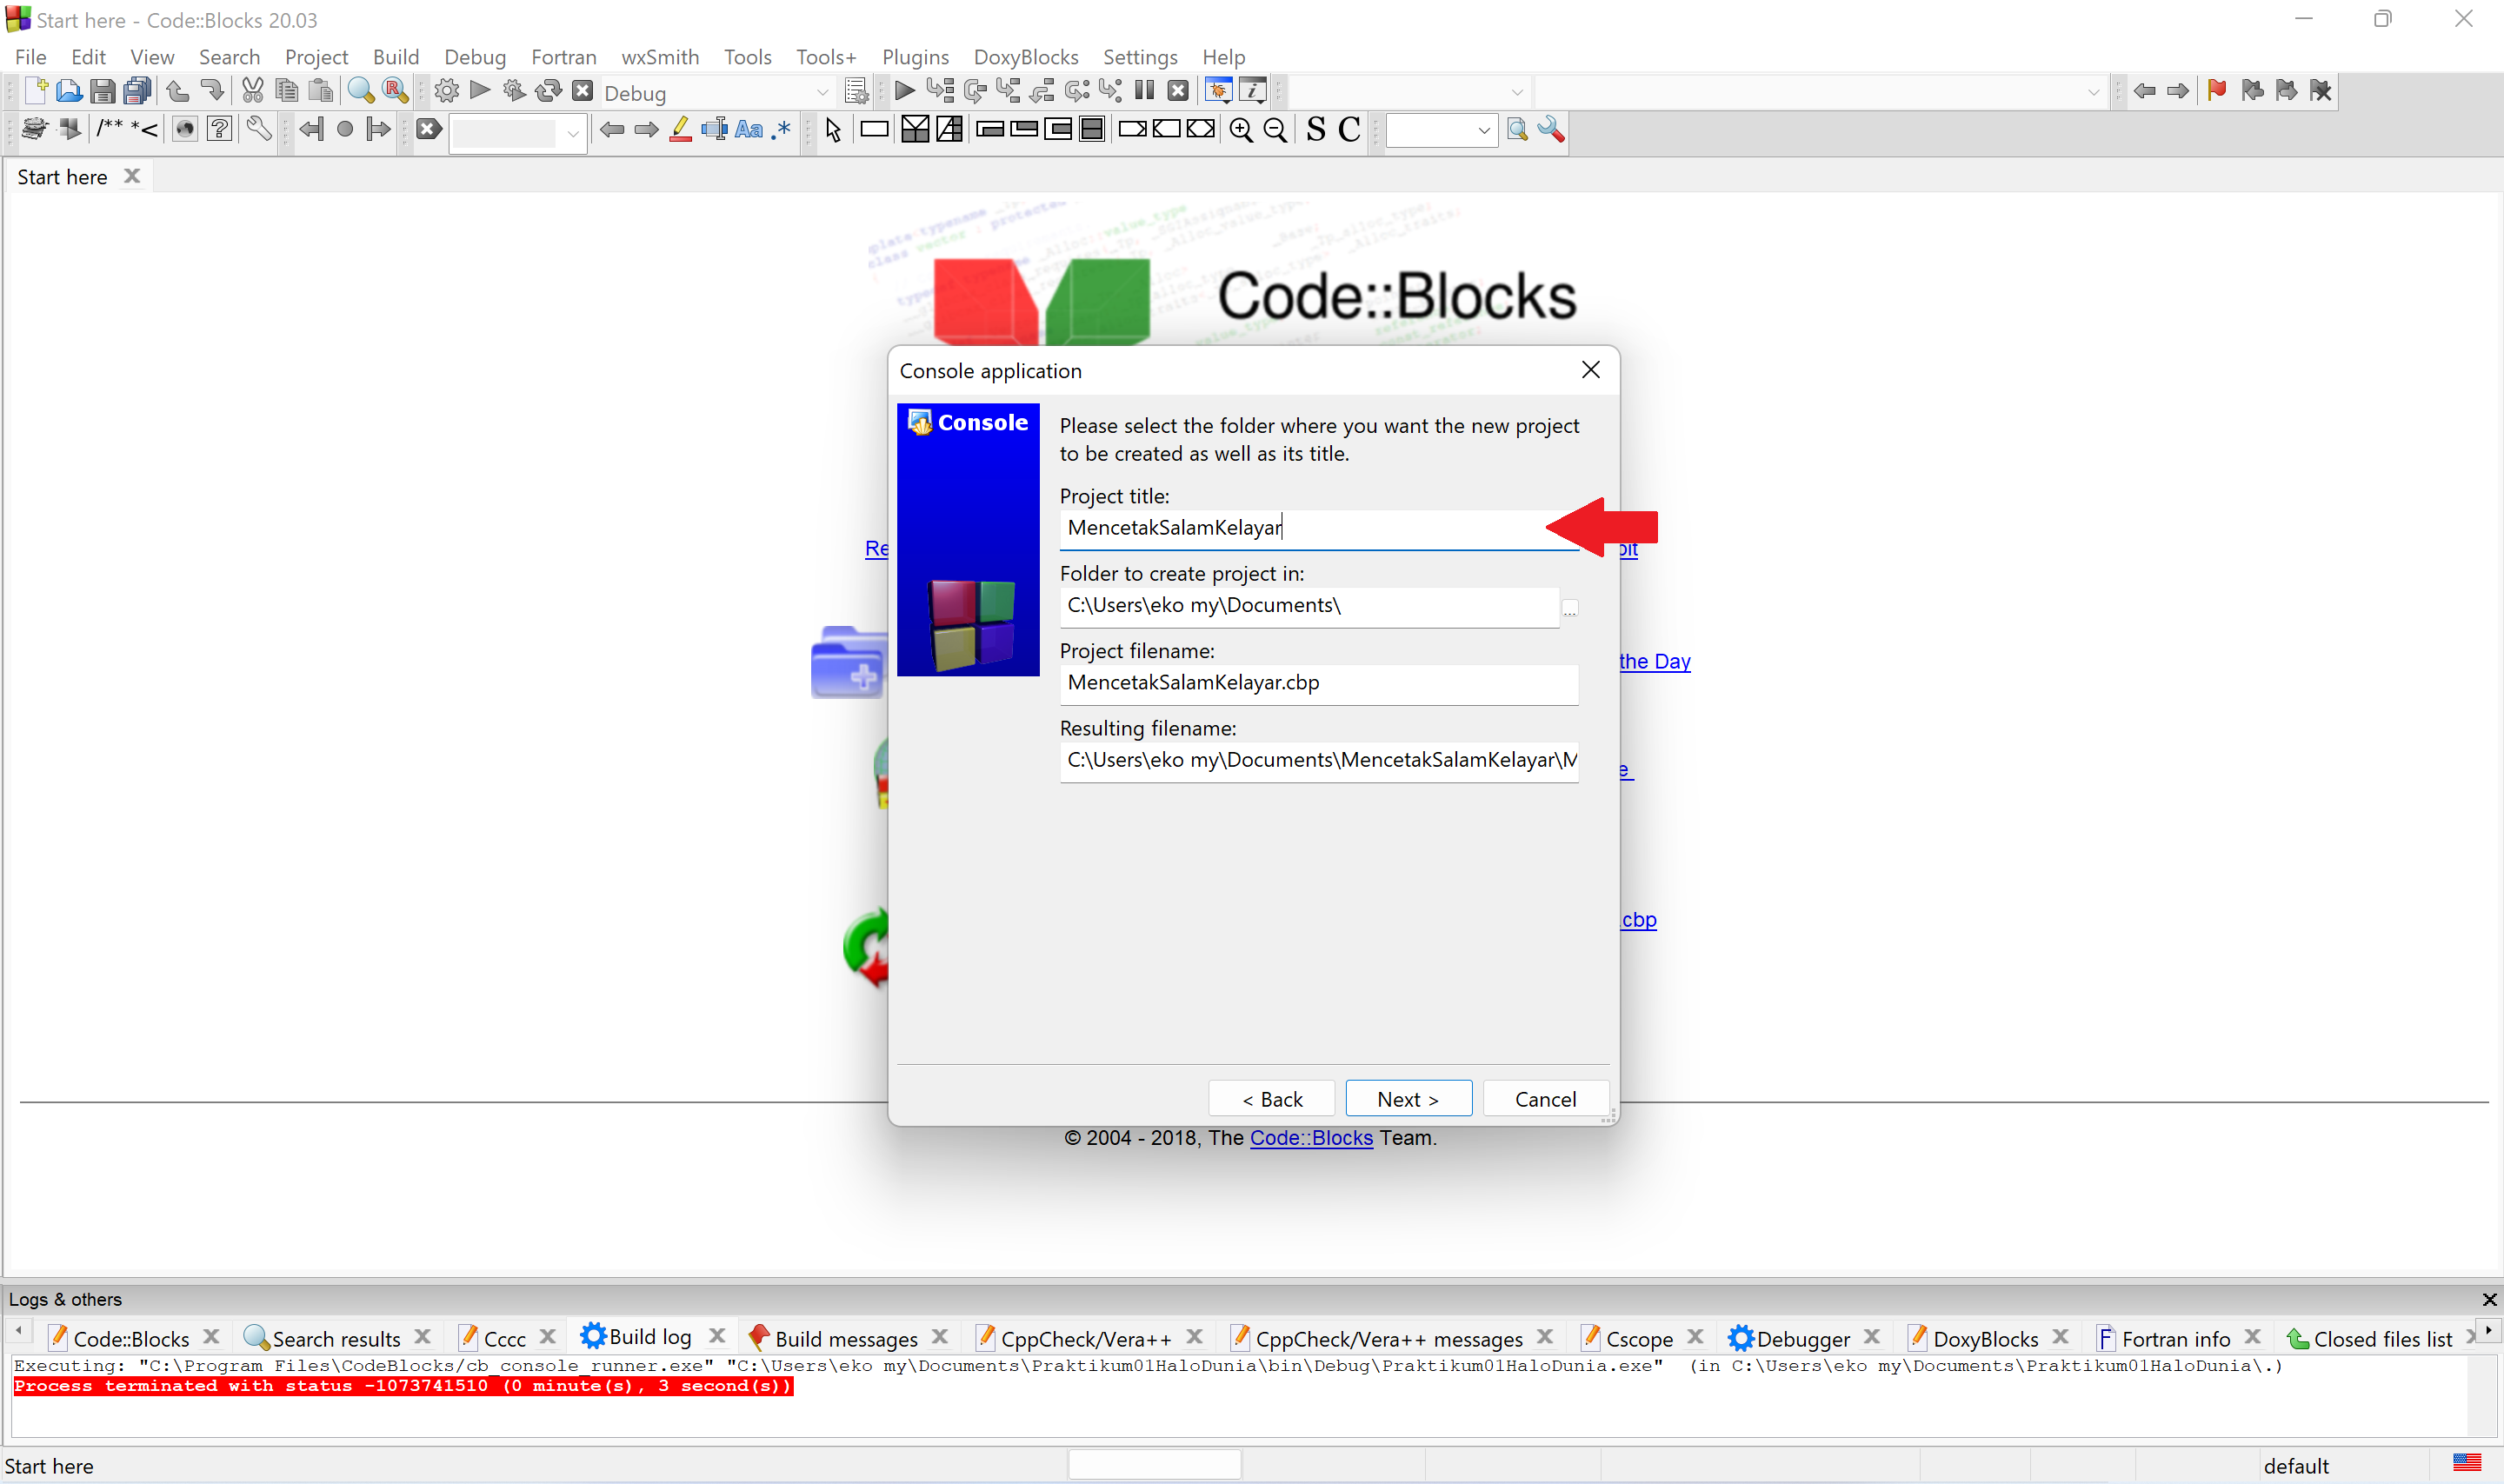
\includegraphics[width=0.7\linewidth]{../P1/img/screenshot006.png}
	\caption{}
	\label{fig:screenshot006}
\end{figure}
\item  Pilih compiler (gcc), pilih dirketori untuk menyimpan, dan klik save.
\begin{figure}[H]
	\centering
	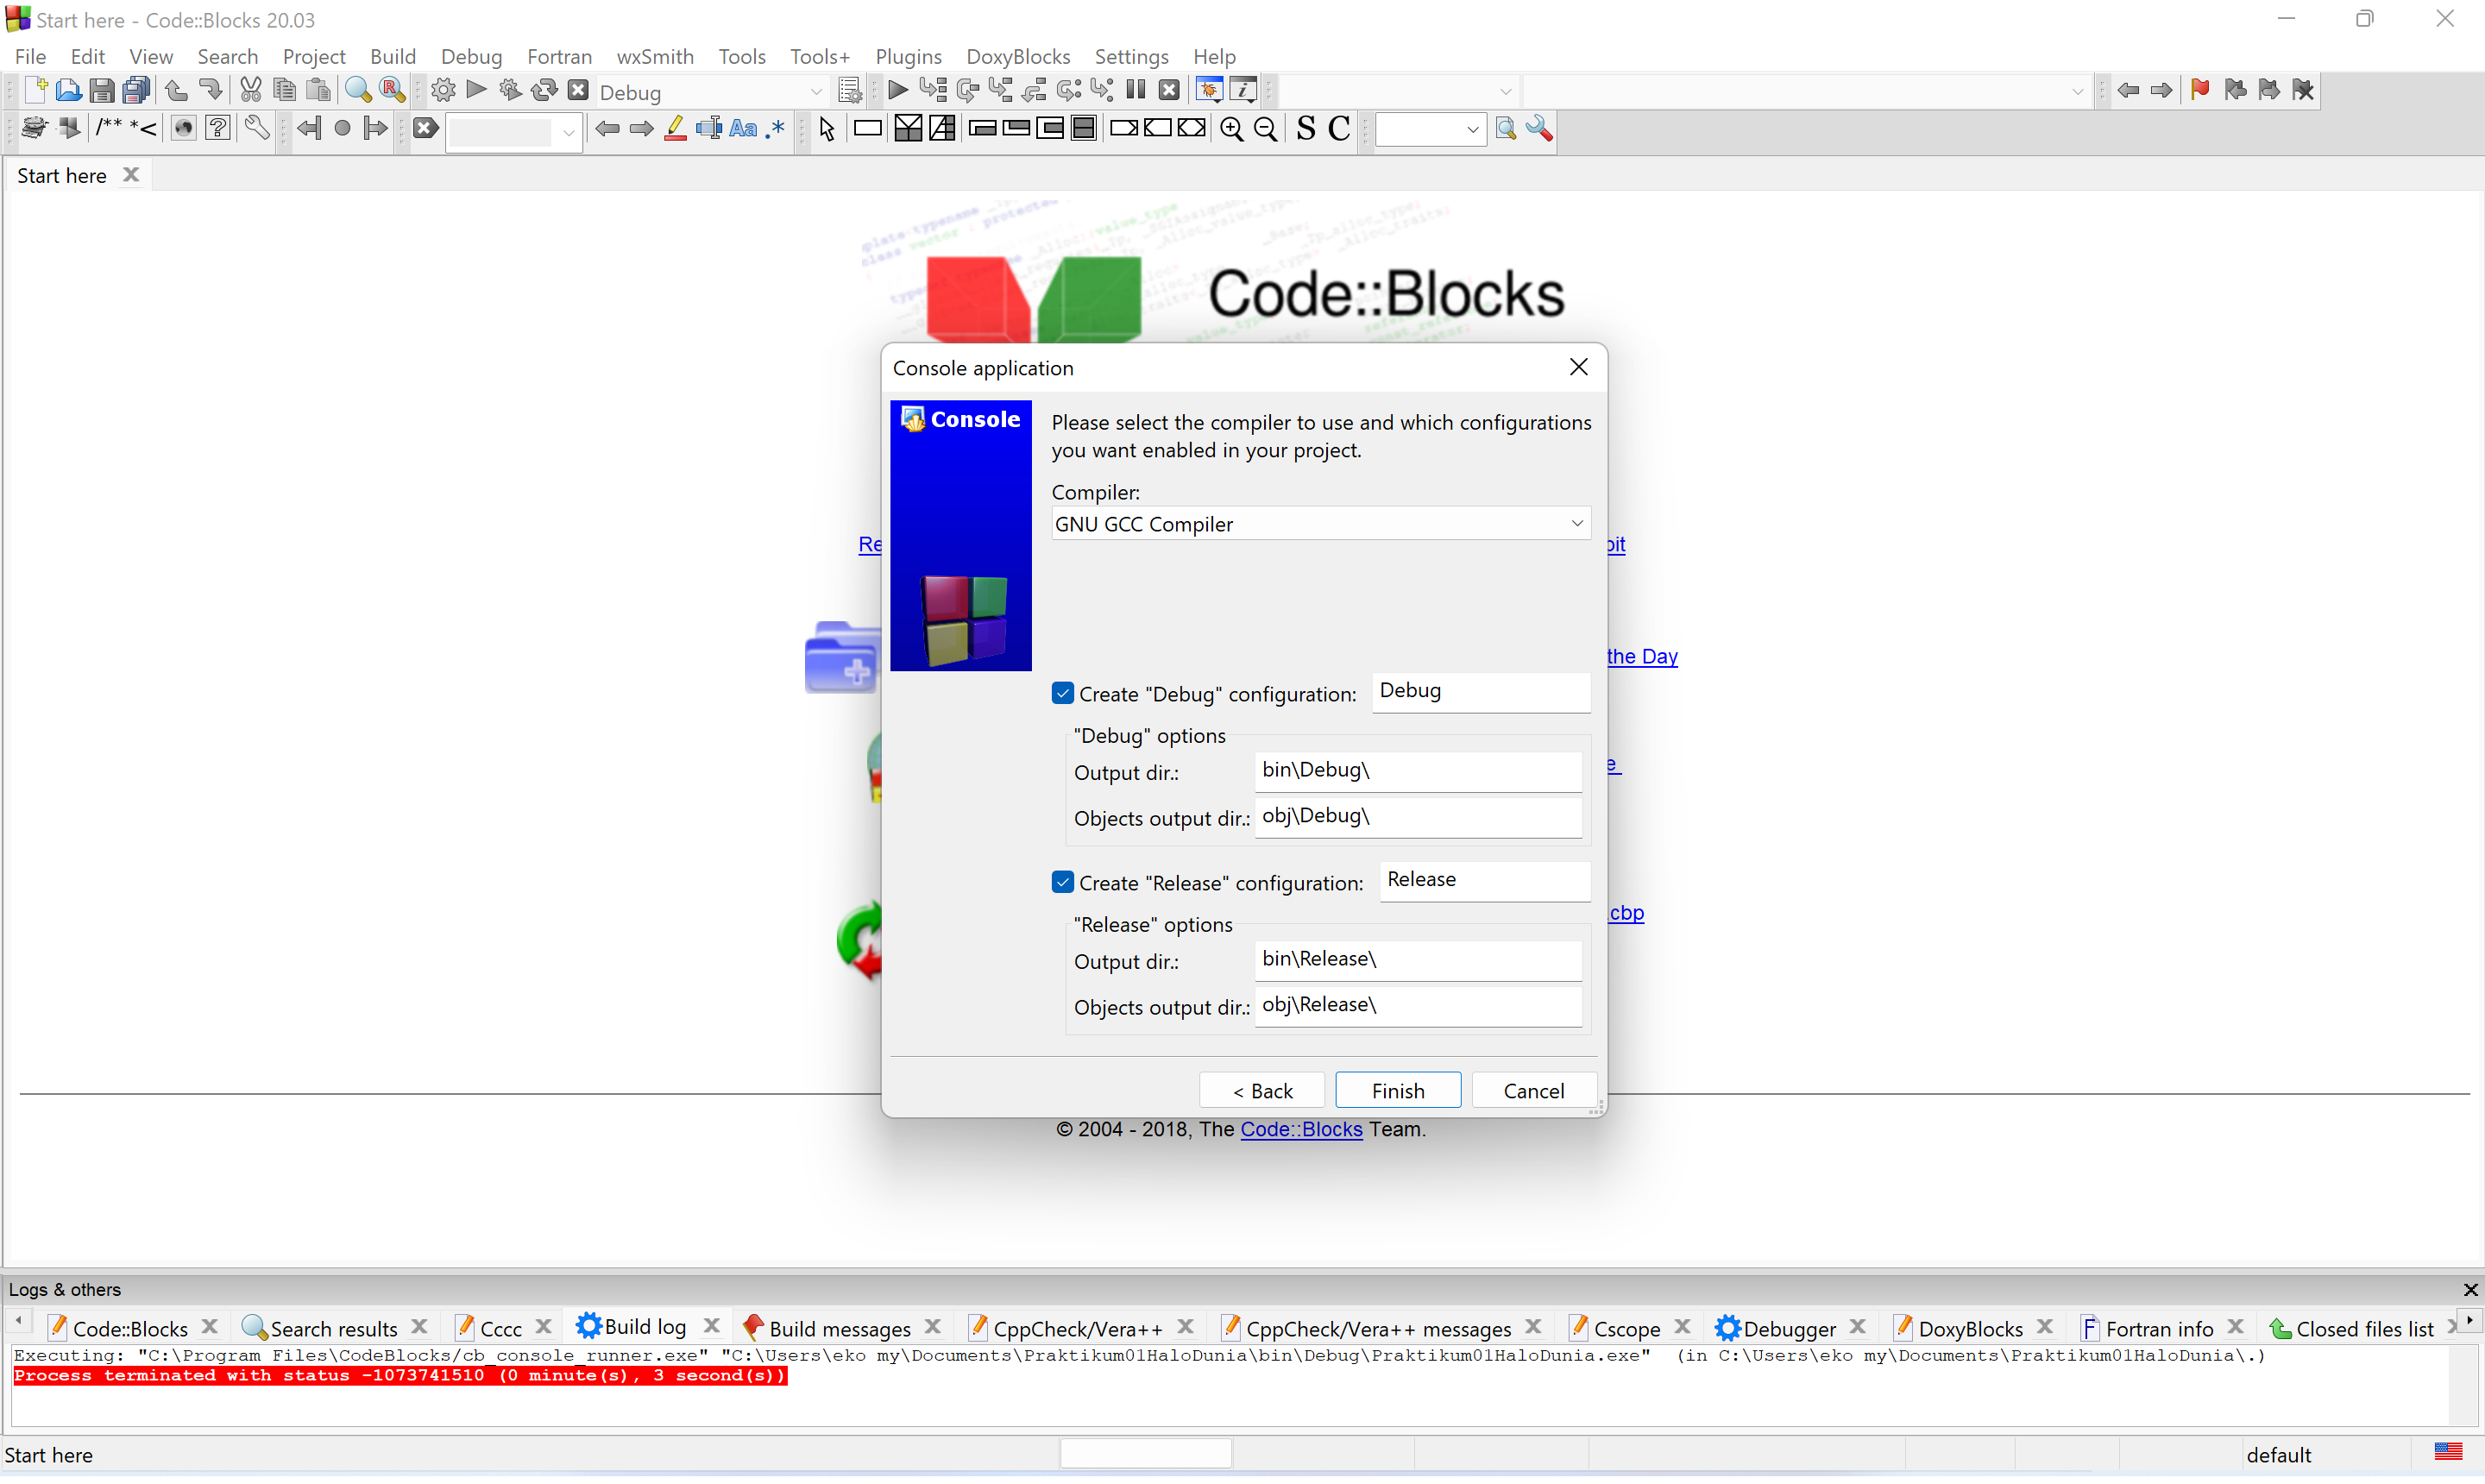
\includegraphics[width=0.7\linewidth]{../P1/img/screenshot007.png}
	\caption{}
	\label{fig:screenshot007}
\end{figure}
\item Ketikan kode pada \ref{fig:screenshot008} ke Code::Blocks 
\begin{figure}[H]
	\centering
	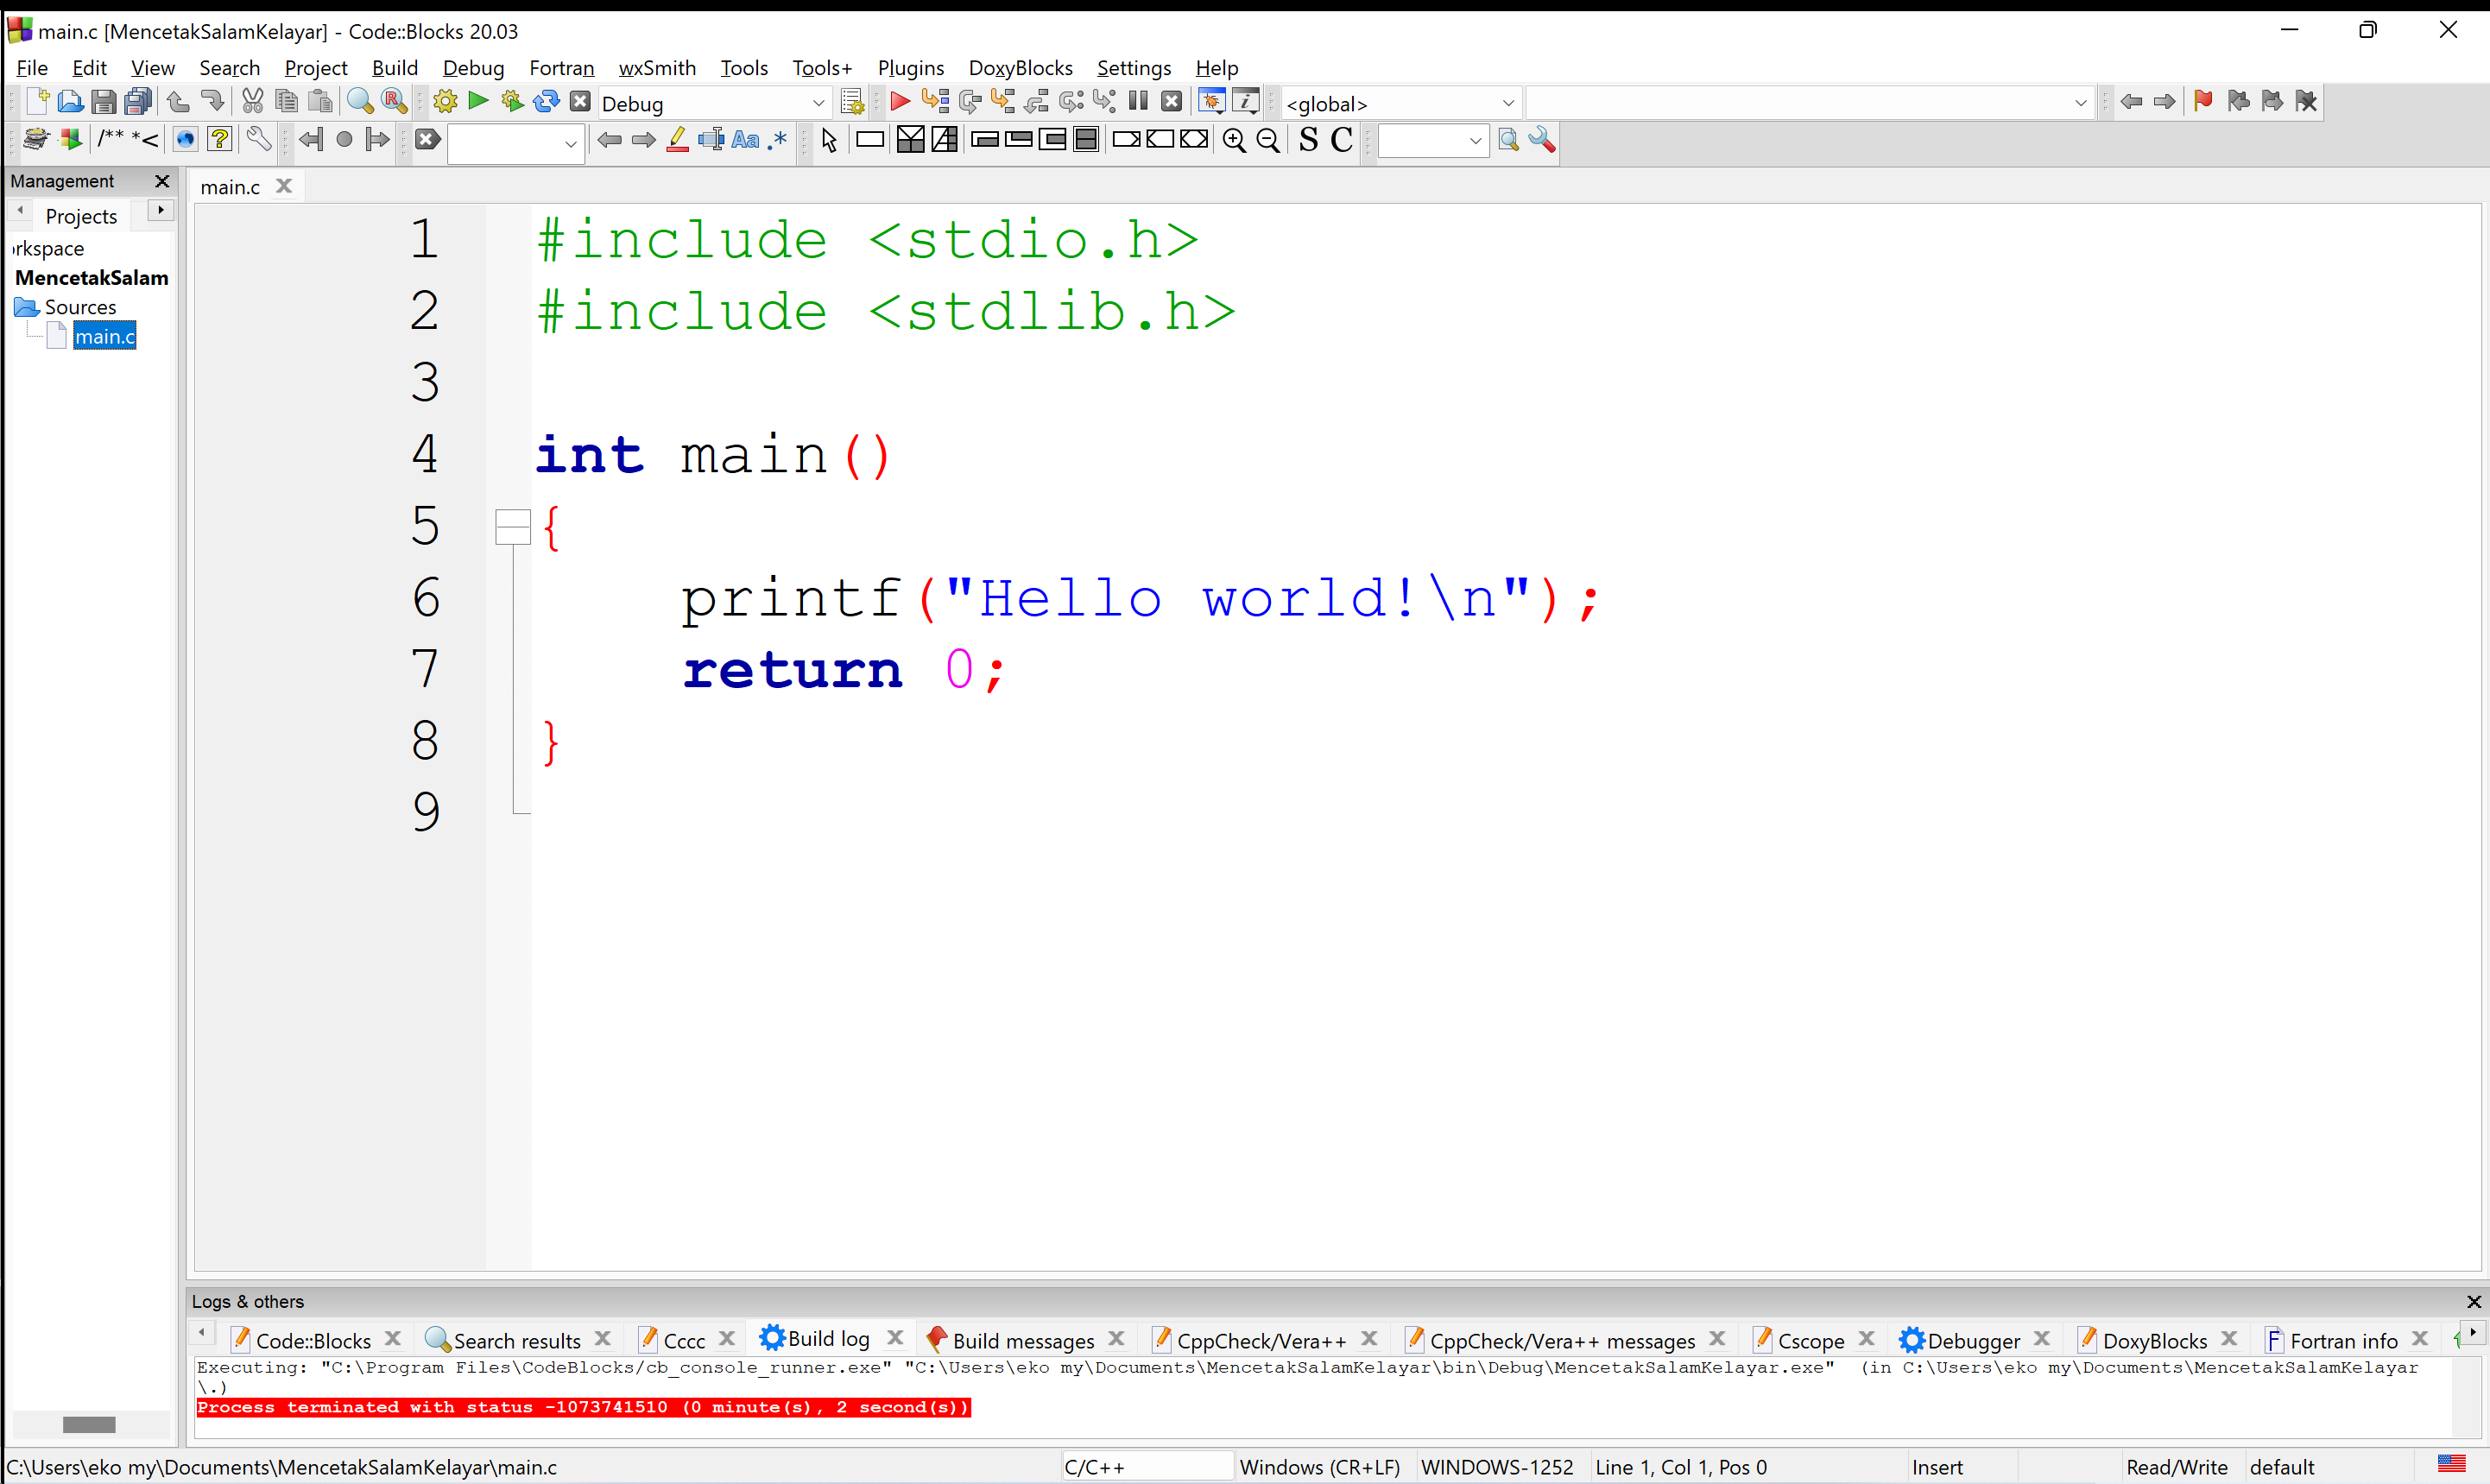
\includegraphics[width=0.7\linewidth]{../P1/img/screenshot008.png}
	\caption{}
	\label{fig:screenshot008}
\end{figure}
\item Klik Build$->$Build and Run atau tekan F9
\begin{figure}[H]
	\centering
	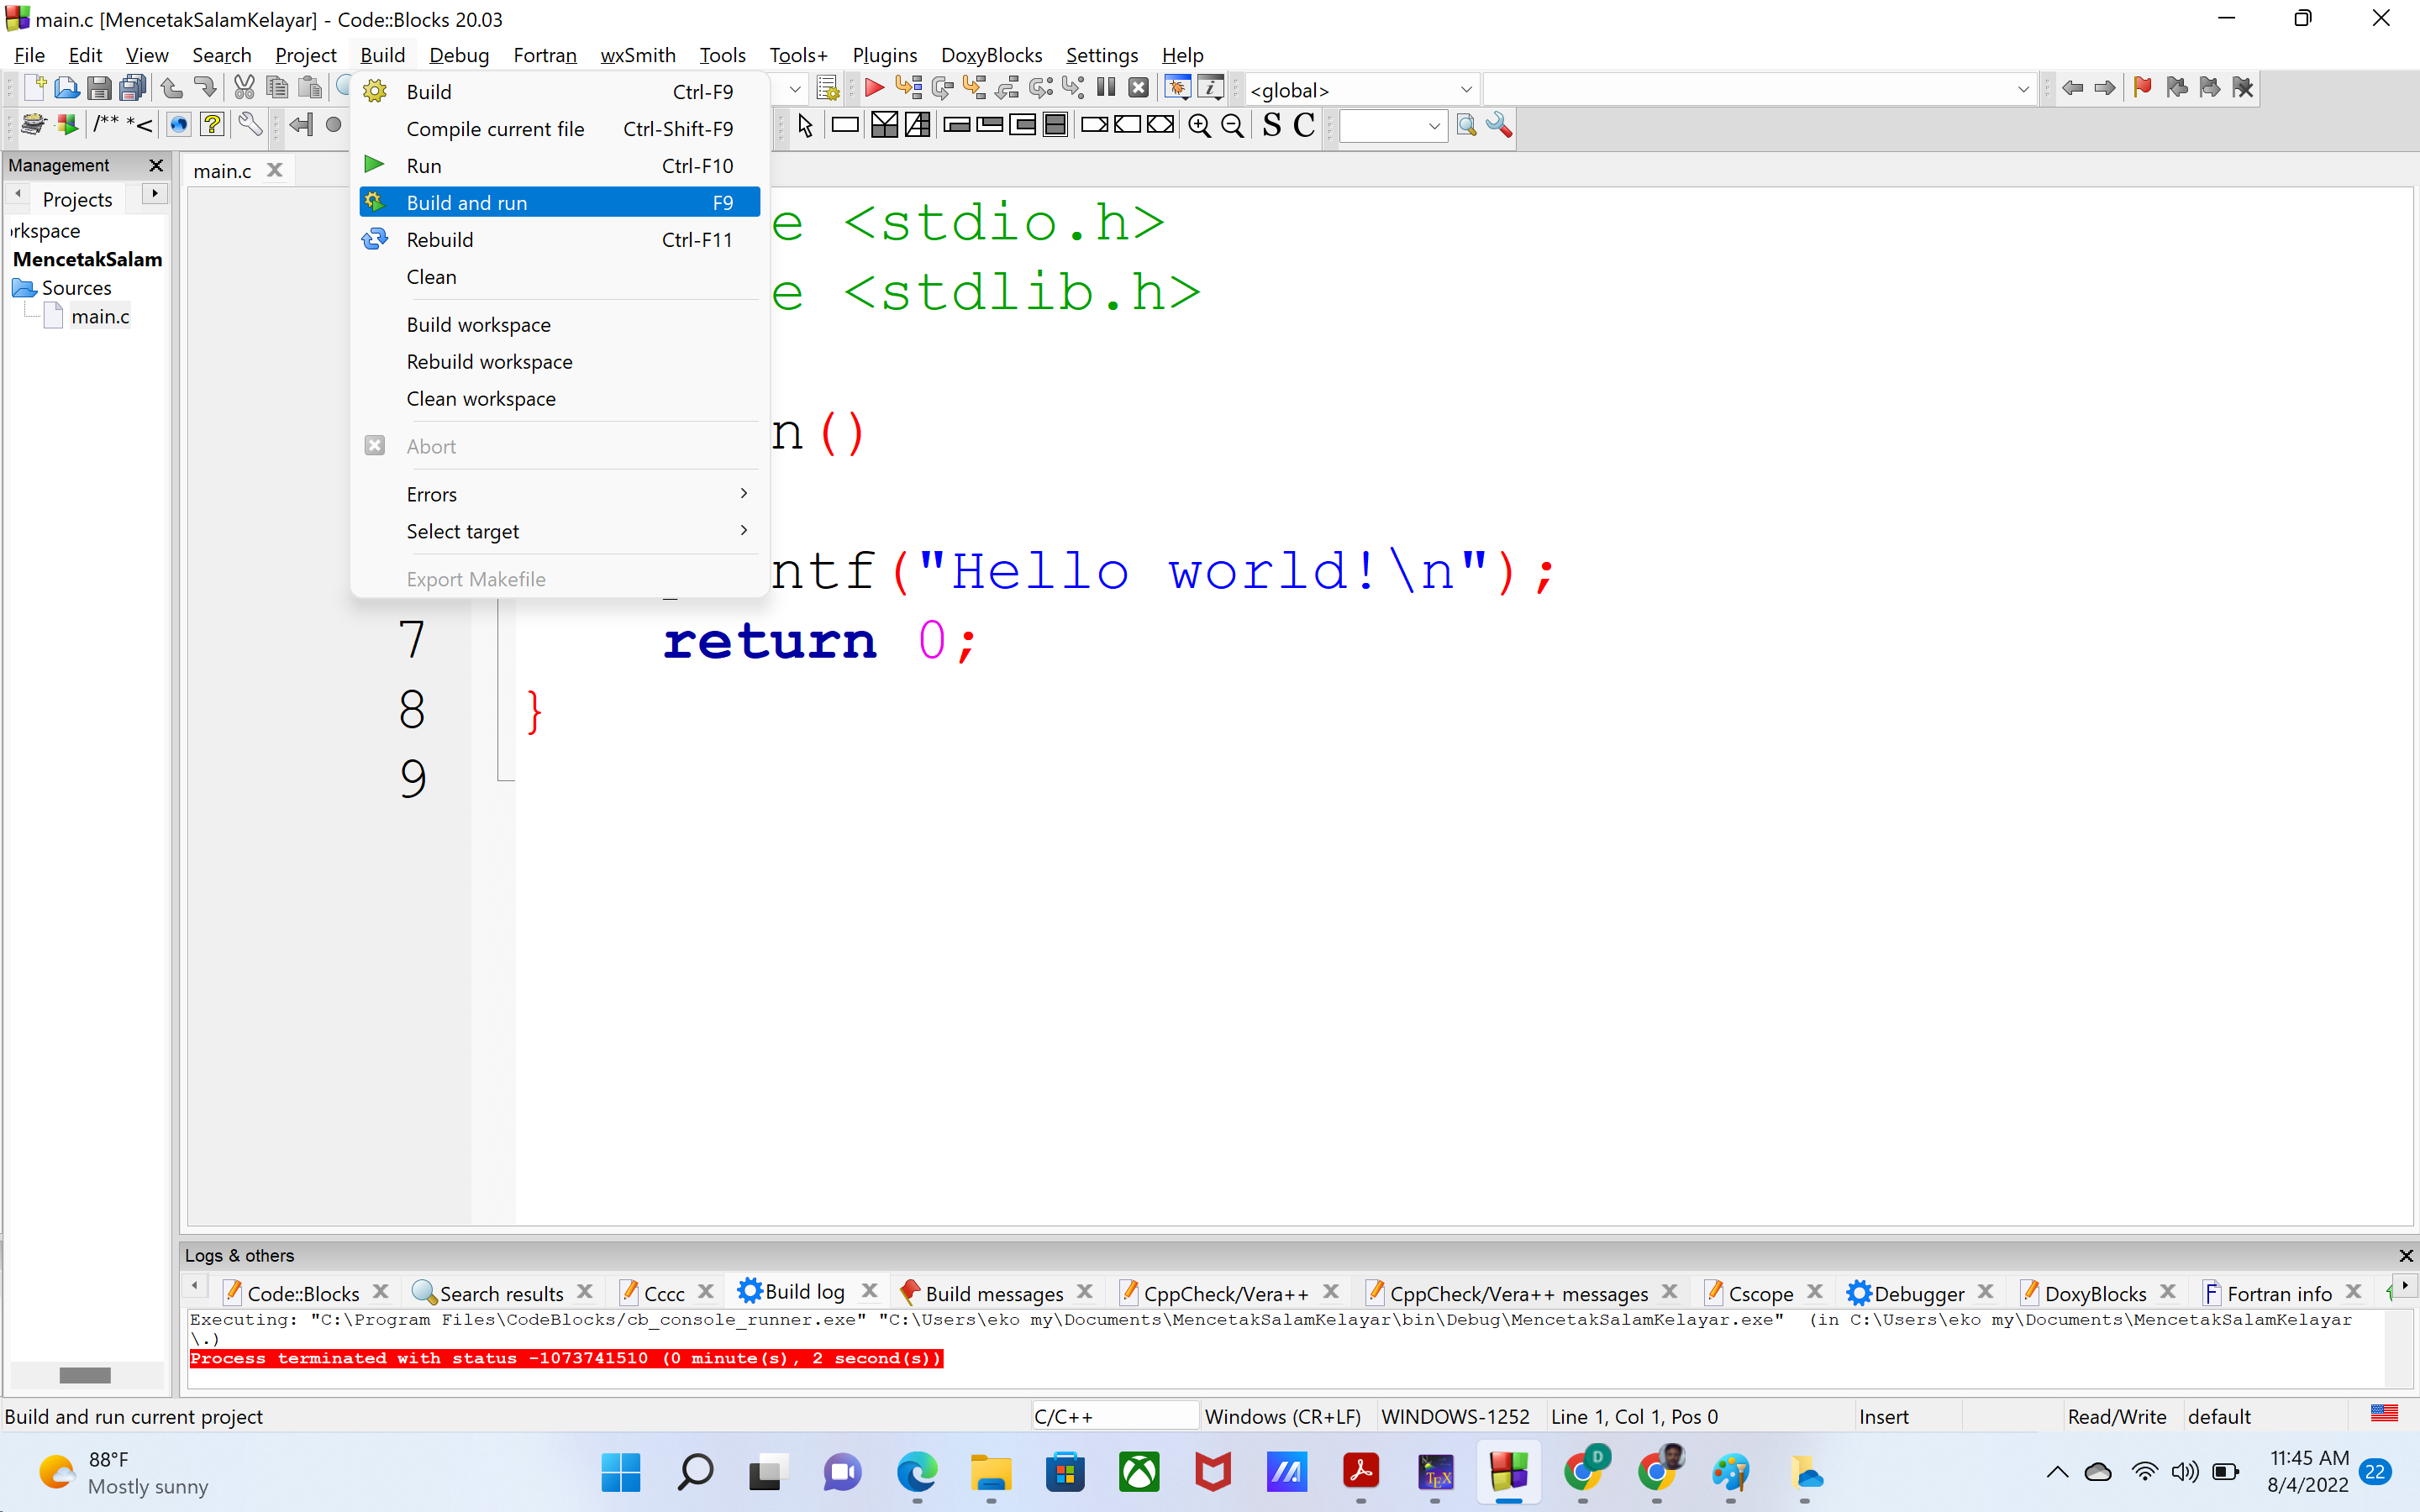
\includegraphics[width=0.7\linewidth]{../P1/img/screenshot009.png}
	\caption{}
	\label{fig:screenshot009}
\end{figure}
% \item The program outputs can be seen on the console.
\item Keluaran dari program dapat dilihat di console
\begin{figure}[H]
	\centering
	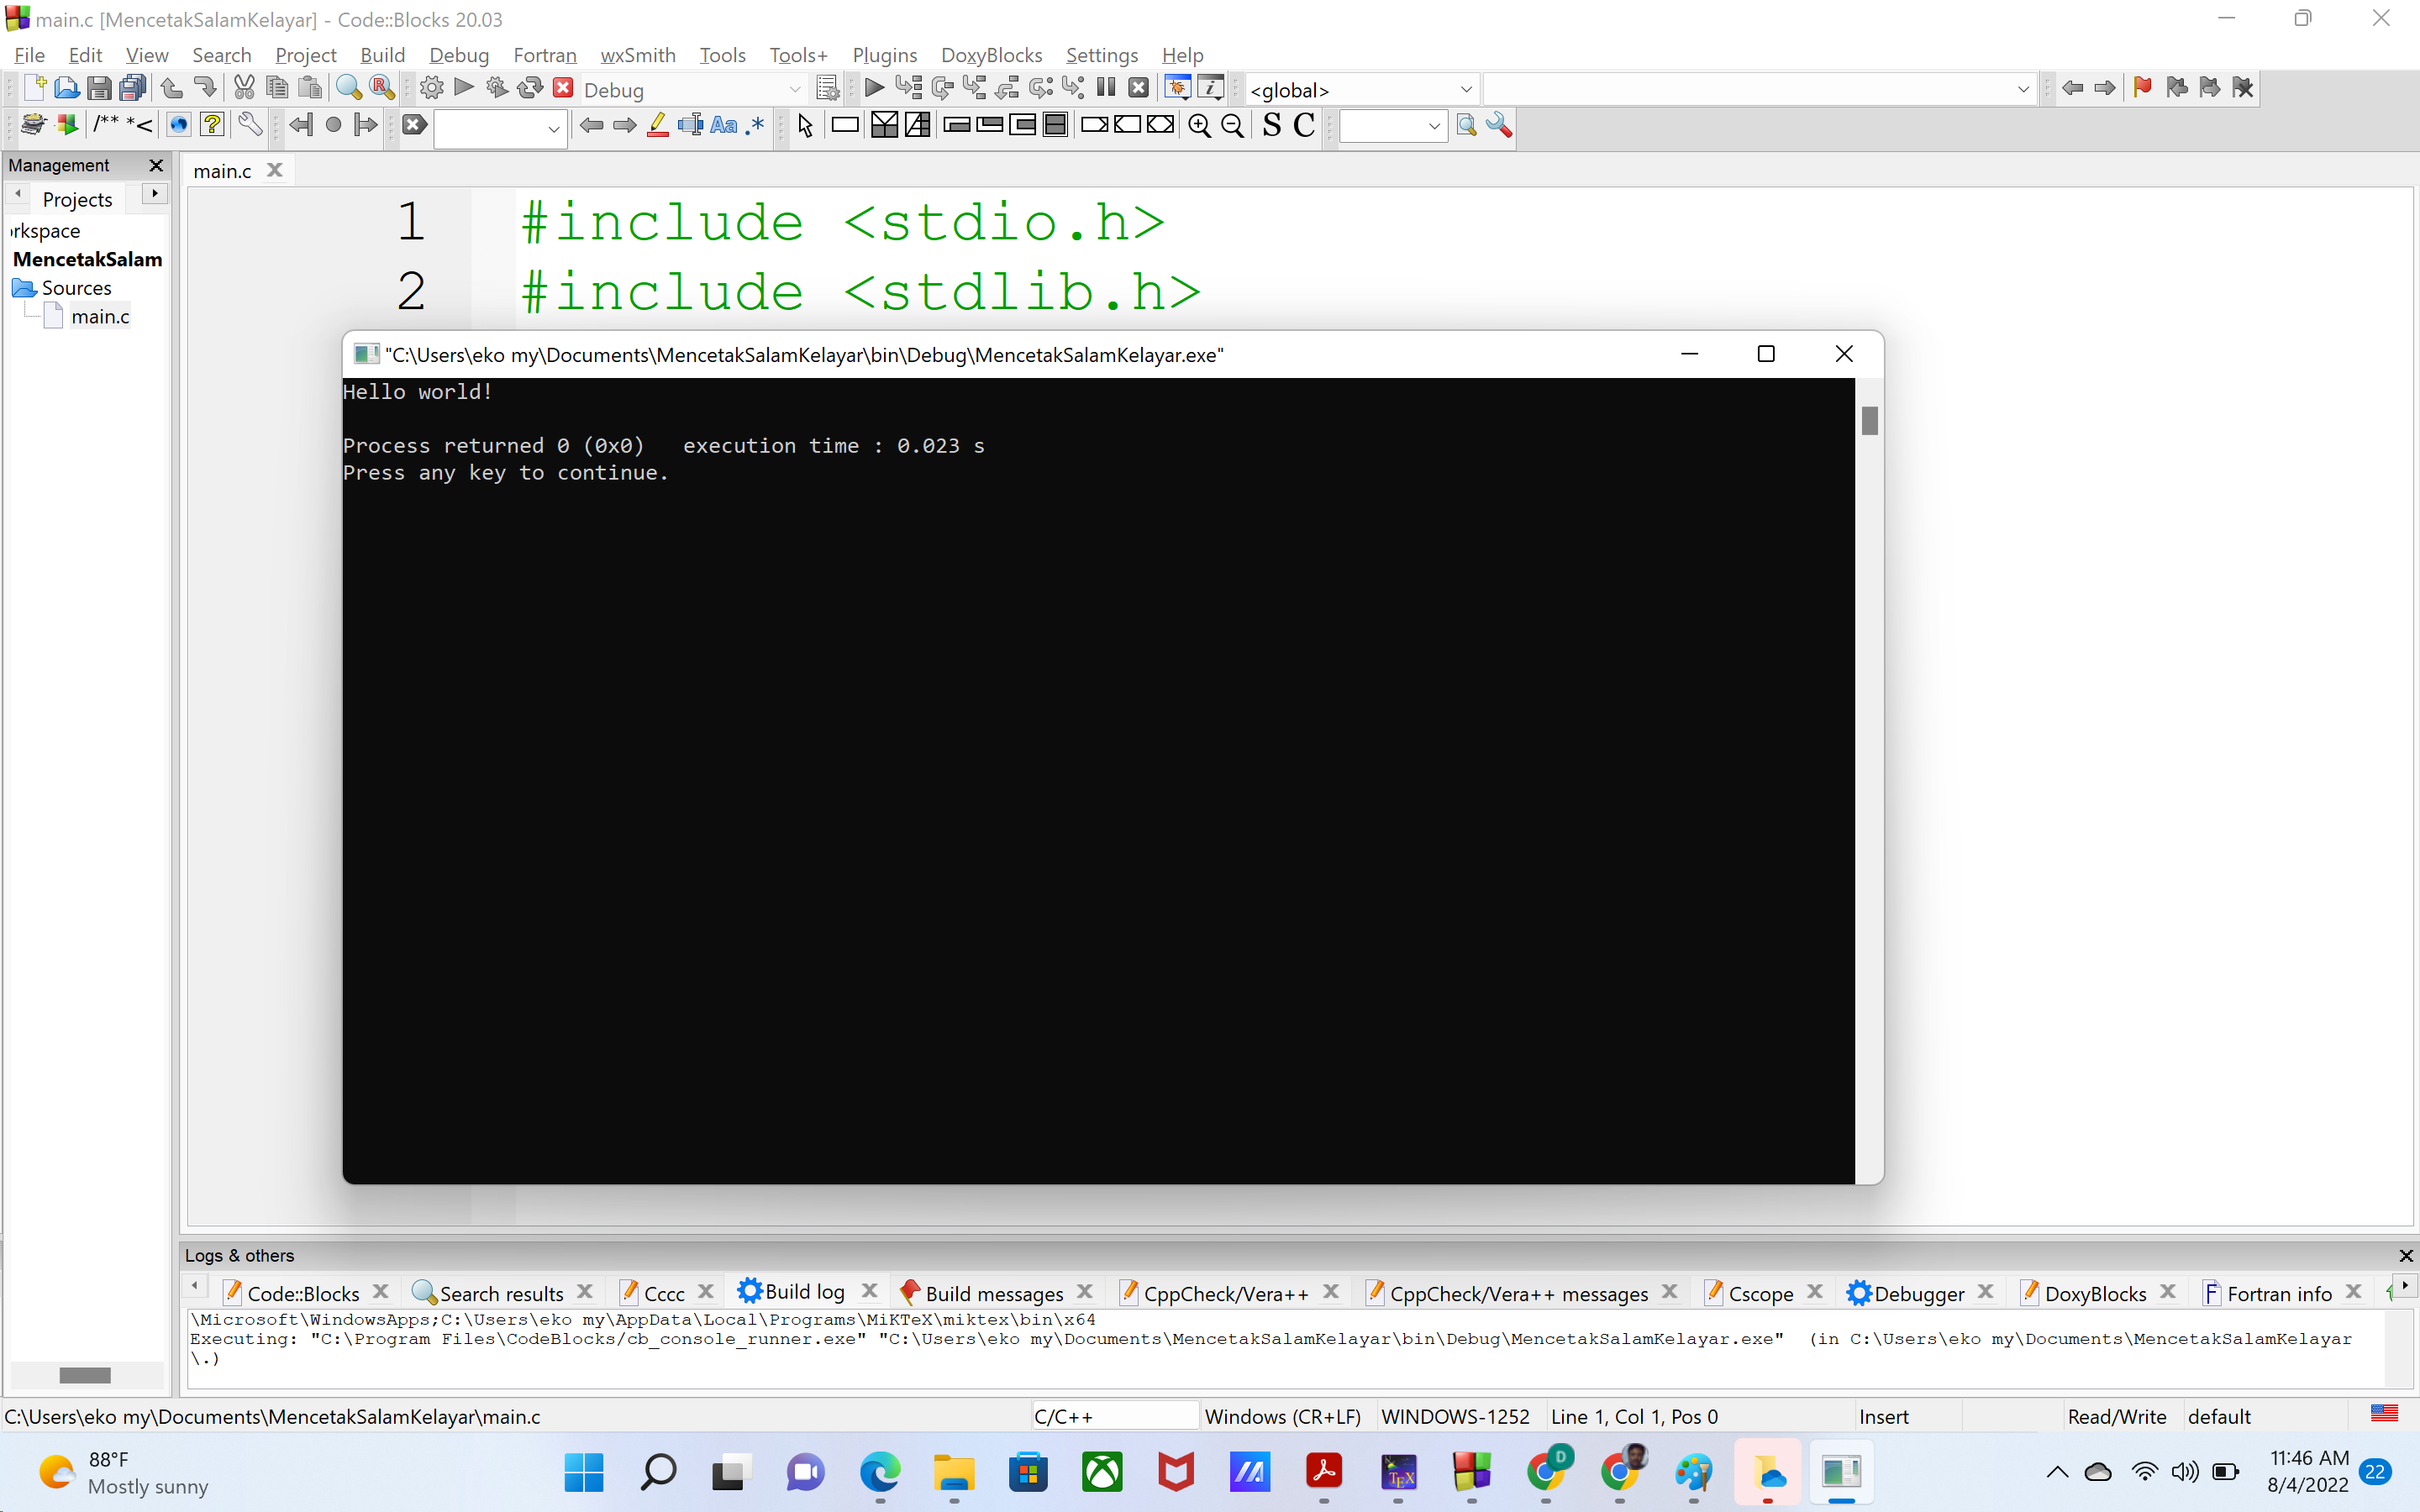
\includegraphics[width=0.7\linewidth]{../P1/img/screenshot010.png}
	\caption{}
	\label{fig:screenshot010}
\end{figure}
\end{enumerate}

% \subsection{Exercise}
% Create a project with name HaloDunia and write the program like can be seen on figure \ref{fig:screenshot008} but change \verb|Hello World!| with \verb|Halo Dunia!|
\subsection{Tugas Pendahuluan}
\begin{enumerate}
	\item Buatlah proyek dengan nama HaloDunia dan tulis program seperti gambar \ref{fig:screenshot008} ubahlah \verb|Hello World!| dengan kata lain!
\end{enumerate}

%\begin{enumerate}
%	\item  Membuat program untuk menampilkan tulisan ke layar.\\
%	Langkah-langkah
%	\begin{enumerate}
%		\item Buatlah project baru dengan nama :\verb*|MencetakTextKeLayar|
%		\item Ketiklah ulang kode pada Listing \ref{lst:mencetaksalamkelayar}
%		\begin{figure}[H]
%		\begin{lstlisting}[language=c,label=lst:mencetaksalamkelayar,caption=Mencetak Teks Kelayar,captionpos=t]
%			/*Mencetak Text ke layar*/
%			
%			#include <stdio.h>
%			
%			int main()
%			{
%				//Mencetak ke layar
%				printf("Saya belajar  Pemprograman Komputer\n");
%				return 0;
%			}
%			
%		\end{lstlisting}
%	\end{figure}
%	\end{enumerate}
%\end{enumerate}
% \section{Structure of C Programming Language}
\section{Struktur Bahasa Pemrograman C}

\begin{lstlisting}[language=c,caption=Contoh program sederhana dalam bahasa C,label=lst:helloworld,captionpos=t]
#include <stdio.h>

int main()
{
	//printing to screen
	printf("Halo Dunia");
	return 0;
}
\end{lstlisting}

% Code on Listing \ref{lst:helloworld} is a simple program to print "Halo Dunia" to screen. The following is the explanation what each line of code do in the program.
Kode pada listing \ref{lst:helloworld} adalah program mudah untuk mencetak "Halo Dunia" ke layar. Berikut penjelasan yang dilakukan setiap baris kode pada program.
\begin{itemize}\setlength\itemsep{-0.1em}
	% \item [Baris 1 :] \verb|#include <stdio.h>|\\ header file library for input and output functions like \verb|printf()| (the one used on line 6)
	% \item[Baris 2 :] Empty line. 
	% \item [Baris 3 :] \verb|int main()|\\ The main function. The main function is the first function to be ran when the program starts.
	% \item[Baris 4 :] \{ \\Beginning of the \verb|main()| function code block.
	% \item[Baris 5 :]\verb|//printing to screen|\\ Comments. Comments are used to explain what the program is doing. Comments are ignored by the program, but helps the reader.
	% \item[Baris 6 :]\verb|printf("Halo Dunia");|\\ Printing "Halo Dunia" to the screen.
	% \item[Baris 7 :] \verb|return 0;| \\Returning the \verb|main()| function (A function ends when it returns)
	% \item [Baris 8 :] \}\\Closing the \verb|main()| function code block.

	\item [Baris 1 :] \verb|#include <stdio.h>|\\ file library header untuk fungsi input dan output seperti \verb|printf()| (contoh digunakan di baris 6)
	\item[Baris 2 :] Baris kosong. 
	\item [Baris 3 :] \verb|int main()|\\ Fungsi main. Fungsi utama adalah fungsi pertama yang akan dijalnkan ketika program dimulai.
	\item[Baris 4 :] \{ \\Permulaan dari \verb|main()| fungsi code block.
	\item[Baris 5 :]\verb|//printing to screen|\\ Komen. Komen digunakan untuk menjelaskan program. Komen akan diabaikan oleh program, tetapi membantu pembaca.
	\item[Baris 6 :]\verb|printf("Halo Dunia");|\\ Print/mencetak "Halo Dunia" ke layar.
	\item[Baris 7 :] \verb|return 0;| \\Mengembalikan \verb|main()| fungsi (sebuah fungsi berakhir ketika dikembalikan/return)
	\item [Baris 8 :] \}\\Menutup \verb|main()| fungsi code block.

\end{itemize}
% \subsection{Exercise}
% Try to swap line 6 and line 7 in Listing \ref{lst:helloworld}. What happened?\\
% What if \verb|return 0;| replaced with \verb|return 1;|?
\subsection{Tugas Pendahuluan}
\begin{enumerate}
	\item Cobalah untuk menukar baris 6 dan baris 7 di listing \ref{lst:helloworld}. Apa yang terjadi? Jelaskan!
	\item Bagaimana jika \verb|return 0;| diganti dengan \verb|return 1;|?
\end{enumerate}


\section{Tipe Data dan Variabel}
\subsection{Tipe Data}
Pada bahasa C, terdapat beberapa tipe data untuk merepresentasikan data yang berupa bilangan bulat, bilangan real, karakter, string, dan lain-lain. Berikut adalah beberapa tipe data pada C.
% In C programming language, there are several data types to represent integer, real number, characters, string, and etc.
\begin{center}
    \captionof{table}{Beberapa tipe data di C \label{tab:tipedata}}
	% \begin{tabular}{|l|l|l|}
	% 	\hline
	% 	Data Types & Size         & Description                                         \\ \hline
	% 	int       & 2 or 4 bytes & saves integers                        \\ \hline
	% 	float     & 4 bytes      & saves real numbers to 8 digit behind decimal point. \\ \hline
	% 	double    & 8 bytes      & saves real numbers to 15 digits behind decimal point. \\ \hline
	% 	char      & 1 byte       & saves a character                     \\ \hline
	% \end{tabular}
	\begin{tabular}{|l|l|l|}
		\hline
		Tipe Data & Ukuran       & Deskripsi                                         \\ \hline
		int       & 2 atau 4 bytes & menyimpan integers.                        \\ \hline
		float     & 4 bytes      & menyimpan bilangan real (8 digit dibelakang desimal). \\ \hline
		double    & 8 bytes      & menimpan bilangan real (15 digit dibelakang desimal). \\ \hline
		char      & 1 byte       & menyimpan sebuah karakter.                     \\ \hline
	\end{tabular}
\end{center}
Untuk menampilkan data pada layar, setiap tipe data memiliki format specifier yang dapat digunakan pada formatted string. Berikut adalah format specifier untuk beberapa tipe data.
% To show the data on screen, every data type has a format specifier that can be used on formatted string. The following is the format specifier for several data types.
\begin{center}
    \captionof{table}{Format Specifier \label{tab:formatspecifier}}
	\begin{tabular}{|l|l|}
		\hline
		Format Specifier & Tipe Data   \\ \hline
		\%d or \%i       & int          \\ \hline
		\%f              & float        \\ \hline
		\%lf             & double       \\ \hline
		\%c              & char         \\ \hline
		\%s              & string \\ \hline
	\end{tabular}
\end{center}
Masih ada lebih banyak tipe data dari pada yang dituliskan pada Tabel \ref{tab:tipedata}. Tipe-tipe data ini dan spesifikasinya bisa ditemukan dengan mudah di internet.
% There are still more data types that what was written on Table \ref{tab:tipedata}. These data types and its specification can be found easily on the internet.

\subsubsection{Modifier}
Secara garis besar modifier merupakan sebuah kata, frasa atau klausa yang mengubah makna atau menjelaskan kata benda(noun) atau kata kerja (verb) dalam sebuah kalimat. 
Sedangkan modifier dalam bahasa pemrograman dalah sebuah kata kunci atau keyword yang digunakan untuk mengubah perilaku atau sifat suatu elemen dalam program, seperti variabel, fungsi, atau kelas.
Kita menggunakan modifier untuk mengubah range dari tipe data dasar untuk menyesuaikan dengan keperluan pemrograman. Ada empat modifier, yaitu:
\begin{enumerate}
	\item signed \\
	\verb|int value = -10;| (Menggunakan tanda negatif pada variabel bertipe int yang secara default adalah signed integer.)
	\item unsigned \\
	\verb|unsigned int count = 100;|  (Menggunakan variabel unsigned integer untuk menyimpan bilangan bulat positif tanpa tanda.)
	\item long \\ 
	\verb|long population = 7500000000;| (Menggunakan tipe data long untuk menyimpan nilai yang lebih besar daripada tipe data int.)
	\item short \\
	\verb|short temperature = 20;| (Menggunakan tipe data short untuk menghemat memori ketika kita tahu bahwa nilai yang akan disimpan akan relatif kecil.)
\end{enumerate}


\subsection{Variabel}
Variabel merupakan tempat menyimpan data. Mendeklarasikan suatu variabel dapat dilakukan dengan cara sebagai berikut.
\begin{lstlisting}[language=c,caption=Deklarasi Variabel C,label=lst:deklarasivariabel,captionpos=t]
DataType VariableName;
\end{lstlisting}
\subsubsection{Operator Aritmatika dan Penugasan (Assignment)}
Operator penugasan dapat dilakukan pada variabel yang tidak mempunyai \verb*|const| atau merupakan variabel nilai-l. Namun operator aritmatika dapat menerima kedua variabel dengan const atau tidak (nilai-l dan nilai-r).
Tabel di bawah menunjukkan beberapa operator aritmatika di C.
\begin{center}
    \captionof{table}{Operator Aritmatika di C \label{tab:operatoraritmatika}}
	\begin{tabular}{|c|l|c|}
		\hline
		\multicolumn{1}{|l|}{\textbf{Operator}} & \textbf{Nama} & \multicolumn{1}{l|}{\textbf{Contoh}} \\ \hline
		+  & Penambahan &\verb|x + y |  \\ \hline
		-  & Pengurangan &\verb|x = y|   \\ \hline
		*  & Perkalian   & \verb|x * y|  \\ \hline
		/  & Pembagian   & \verb|x/y|  \\ \hline
		\% & Modulo     & \verb|x % y| \\ \hline
	\end{tabular}
\end{center}

Tabel di bawah menunjukkan beberapa operator penugasan.
\begin{center}
    \captionof{table}{Operator Penugasan \label{tab:operatorpenugasan}}
	\begin{tabular}{|c|c|c|}
		\hline
		\multicolumn{1}{|l|}{Operator} & \multicolumn{1}{l|}{Contoh}       & \multicolumn{1}{l|}{Arti yang sama}  \\ \hline
		=   & x = 5   & x = 5      \\ \hline
		+=  & x += 3  & x = x + 3  \\ \hline
		-=  & x -= 3  & x = x - 3  \\ \hline
		*=  & x *= 3  & x = x * 3  \\ \hline
		/=  & x /= 3  & x = x / 3  \\ \hline
		\%= & x \%= 3 & x = x \% 3 \\ \hline
		\&= & x \&= 3 & x = x \& 3 \\ \hline
		|=  & x |= 3  & x = x | 3  \\ \hline
		\textasciicircum{}=            & x \textasciicircum{}= 3           & x = x \textasciicircum 3           \\ \hline
		\textgreater{}\textgreater{}=  & x \textgreater{}\textgreater{}= 3 & x = x \textgreater{}\textgreater 3 \\ \hline
		\textless{}\textless{}=        & x \textless{}\textless{}= 3       & x = x \textless{}\textless 3       \\ \hline
	\end{tabular}
\end{center}
Terdapat juga "singkatan" untuk beberapa operator penugasan seperti \verb*|x+=1| dan \verb*|x-1| yaitu \verb*|++| dan \verb*|--| yang masing-masing disebut kenaikan dan penurunan.
Singkatan ini digunakan seperti berikut.
\begin{verbatim}
    x++;
    x--;
    ++x;
    --x;
\end{verbatim}

\subsubsection{Operator Bitwise}
Bitwise adalah operator khusus untuk menangani operasi logika bilangan biner dalam bentuk bit. \\
Bilangan biner sendiri merupakan jenis bilangan yang hanya terdiri dari 2 jenis angka, yakni 0 dan 1.
Jika nilai asal yang dipakai bukan bilangan biner, akan dikonversi secara otomatis oleh compiler C menjadi bilangan biner. Misalnya 7 desimal = 0111 dalam bilangan biner.
\\
\begin{center}
    \captionof{table}{Operator Bitwise \label{tab:operatorbitwise}}
	\begin{tabular}{|c|c|c|c|c|c|}
	\hline
	\multicolumn{1}{|l|}{Operator} & \multicolumn{1}{|l|}{Nama} & \multicolumn{1}{|l|}{Contoh} & \multicolumn{1}{|l|}{Biner} & \multicolumn{1}{|l|}{Hasil (biner)} & \multicolumn{1}{|l|}{Hasil (decimal)} \\ \hline
	\&                                    & AND                               & 10 \& 12                            & 1010 \& 1100                       & 1000                                       & 8                                            \\ \hline
	|                                     & OR                                & 10 | 12                             & 1010 | 1100                        & 1110                                       & 14                                           \\ \hline
	\textasciicircum{}                    & XOR                               & 10 \textasciicircum 12              & 1010 \textasciicircum 1100         & 0110                                       & 6                                            \\ \hline
	$\sim$                                & NOT                               & $\sim$10                            & $\sim$1010                         & 0101                                       & -11 (two complement)                         \\ \hline
	\textless{}\textless{}                & Left shift                        & 10 \textless{}\textless 1           & 1010 \textless{}\textless 1        & 10100                                      & 20                                           \\ \hline
	\textgreater{}\textgreater{}          & Right shift                       & 10 \textgreater{}\textgreater 1     & 1010 \textgreater{}\textgreater 1  & 101                                        & 5                                            \\ \hline
	\end{tabular}
\end{center}

\begin{center}
	\colorbox{pink}{\parbox{0.8\linewidth}{\textbf{Catatan:} Terdapat beberapa operator dalam Bahasa C. Silahkan pelajari dengan mencari referensi secara mandiri.}}
\end{center}
\subsection{Tugas Pendahuluan}
\begin{lstlisting}[language=c,caption=Menggunakan operator penugasan pada variabel const,label=lst:constassignment,captionpos=t]
#include <stdio.h>
int main()
{
    //deklarasi variabel const
    const int x=0;
    x=1;
	return 0;
}
\end{lstlisting} 
% Try to compile the program in Listing\ref{lst:constassignment}, what happened?
Coba jalankan program di Listing \ref{lst:constassignment}, apa yang terjadi?


\section{Output dan Input}

\subsection{printf()}
\verb*|printf|  digunakan untuk mencetak string  ke output yang dilengkapi dengan format specifier yang dimulai dengan \verb*|%| pada string.
% is a function in C that is used to print formatted string.
% You can use format specifier within the formatted string to outputs your variables.

\begin{verbatim}
	printf(const char *format,v1,v2,..,vn)
\end{verbatim}

Format specifier untuk beberapa tipe data dapat dilihat pada Tabel \ref{tab:formatspecifier}
% The format specifier for each data types can be seen on Table \ref{tab:formatspecifier}


\begin{description}
	\item[Contoh \thesubsection.1]  Mencetak teks ke layar.
	\begin{lstlisting}[language=c,caption = Mencetak Tulisan "C Programming" Ke layar,captionpos=t]
		#include <stdio.h>    
		int main()
		{ 
			// Mencetak teks yang ditulis dalam simbol "
			printf("C Programming");
			return 0;
		}
	\end{lstlisting}
	\begin{itemize}
		\item Seluruh program C harus berisi fungsi main() tempat program memulai menjalankan kode. 
		% \item All C program must have main() function where the program needs to run the code.
		\item Fungsi \verb*|printf()| adalah library untuk mengirim output yang telah diformat ke layar.  Fungsi \verb*|printf()|  mencetak string dalam tanda dua tanda petik. 
		% \item \verb*|printf()| function is a function from stdio.h library. This function outputs the string inside the symbol " to the screen.
		% \item \verb*|return 0;| statement in the \verb*|main()| function tells the program to exit.
		\item \verb*|return 0;| pernyataan di \verb*|main()| fungsi memberitahu program untuk keluar.
	\end{itemize}
	\item [Contoh \thesubsection.2] Mencetak integer.
	\begin{lstlisting}[language=c,captionpos=t]
		#include <stdio.h>
		int main()
		{
			int testInteger = 5;
			printf("Number = %d", testInteger); // <- %d format string
			return 0;
		}
	\end{lstlisting}
	
	
	Pada contoh ini digunakan format specifier \verb*|%d| untuk mencetak tipe data \verb*|int|. \verb*|%d| pada tex akan digantikan oleh isi dari \verb*|testInteger|. 
	% The code above uses the format specifier \verb*|%d| to prints \verb*|int| data type. The \verb*|%d| part of the string will be replaced with the value of \verb*|testInteger|.

	\item[Contoh \thesubsection.3] Keluaran bilangan real (float atau double)
	\begin{itemize}\label{eq:LuasSegitiga}
		\item \verb|Base|  : menggunakan \verb|float| tipe data.
		\item \verb|Height|: menggunakan \verb|float| tipe data.
		\item \verb|Area|  : menggunakan \verb|float| tipe data.
		\begin{equation}
			Luas = \frac{1}{2} \times Alas \times Tinnggi
		\end{equation}
	\end{itemize}
	\begin{lstlisting}[language=c,captionpos=t]
		#include <stdio.h>
		
		int main()
		{
			// deklarasi variabel
			float Base;
			float Height;
			float Area;
			// inisialisasi nilai
			Base = 10;
			Height = 5;
			// menghitung area
			Area = 0.5*Base*Height;
			// mencetak area ke layar
			printf("Area = %f",Area);
			return 0;
		}
		
	\end{lstlisting}
	
	Penjelasan
	\begin{description}
		\item[Baris 6-8]  \verb|Alas|, \verb|Tinggi| dan \verb|Luas| bertipe data \verb|float| untuk menyimpan data parameter luas segitiga.
		\item[Baris 10 dan 11] Memberi nilai ke Variabel \verb|Alas|=10 dan \verb|Tinggi|=5
		\item[Baris 13] Menghitung luas alas sesuai dengan persamaan \ref{eq:LuasSegitiga}
		\item[Baris 15] Mencetak \verb|Luas| ke layar dengan menggunakan perintah \verb|printf|.
	\end{description}
\end{description}

.\subsection{scanf}
Fungsi  \verb*|scanf(const char *format, ...)| membaca input dengan format.
% \verb*|scanf(const char *format, ...)| reads input according to the format string.

\begin{enumerate}
	\item Syntax 
	\begin{verbatim}
		scanf(const char *format, ...)
	\end{verbatim}
	\item Parameter \\
	% Format string in C consist of one or more whitespace, non-whitespace, and format specifiers.
	Format string pada C yang terdiri dari satu atau lebih yang terdiri dari \\
	Karakter Whitespace,Karakter Non-whitespace  dan  Format specifiers. 
	\item Return Value \\
	Ketika berhasil maka fungsi mengembalikan jumlah item dari argumen yang berhasil di baca.
	% The function will return the number of arguments it has sucessfully read.
	
\end{enumerate}

\begin{description}
	\item  [Contoh \thesubsection.4] Menghitung luas segitiga dengan  dengan alas \verb*|Alas|   dan tinggi \verb*|Tinggi| yang diinputkan dari keyboard. 
	\begin{lstlisting}[language=c]
#include <stdio.h>

int main()
{
	float Alas ,Tinggi,Luas;
	
	printf("Menghitung luas segitiga\n");
	printf("\nMasukkan Alas= ");
	scanf("%f",&Alas);
	printf("\nMasukkan Tinggi=");
	scanf("%f",&Tinggi);
	Luas = 0.5*Alas *Tinggi;
	printf("Luas Seigtiga = %.2f", Luas);
	return 0;
}
	\end{lstlisting}
\begin{figure}[H]
	\centering
	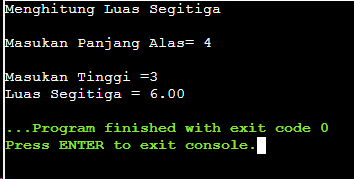
\includegraphics[width=0.5\linewidth]{../P1/img/screenshot0005.png}
	\caption{}
	\label{fig:screenshot0005}
\end{figure}

\begin{description}
	\item [Baris 9]\verb|scanf("%f",&Alas);| meminta masukan untuk alas segitiganya
	\item [Baris 11]\verb|scanf("%f",&Tinggi);| meminta masukan tinggi segitiganya
	\item [Baris 13]\verb|printf("Triangle Area = %.2f", Luas);|,  \verb|.2| si \verb|%.2f| menandakan bahwa hanya 2 angka di belakang koma(decimal point) yang perlu dicetak.
\end{description}

	\item[Contoh \thesubsection.5] Program untuk memasukkan nama dan email.\\
	Pada contoh ini dipelajari bagaimana cara menginputkan string atau text dari keyboard dan mencetak kelayar. Input dari contoh program ini ada dua yang terdiri dari \verb|snama| dan \verb|sAlamatEmail|. Oleh karena text berisi banyak karakter maka masing-masing variabel dideklarasikan sebagai kumpulan karakter dengan jumlah karakter untuk sNama=20 dan sAlamatEmail=30. 
	% This example shows how to input string or text from keyboard and outputs it on the screen. Input from this program consist of \verb|sName| and \verb|sEmail|.
	\begin{figure}[H]
	\begin{lstlisting}[language=c]
		#include <stdio.h>
		
		int main () 
		{
			char sName[20], sEmail[30];
			
			printf("Masukkan Nama: ");
			scanf("%19s", sName);
			
			printf("Masukkan Email: ");
			scanf("%29s", sEmail);
			
			printf("Nama : %s\n", sName);
			printf("Email:%s", sEmail);
			return(0);
		}
	\end{lstlisting}
\end{figure}
\end{description}


\subsection{Escape Sequence}
Escape Sequence adalah urutan karakter yang digunakan untuk memformat output dan tidak ditampilkan ketika dicetak ke layar. Setiap karakter mempunyai fungsi tertentu. 
% Some characters can't be written on the format string because they are used to format the outputs.
% So, to outputs those special characters we use escape sequences.

\begin{table}[H]
	\centering
	\captionof{table}{Escape Sequence \label{tab:escapesequence}}
	\begin{tabular}{|l|l|l|}
		\hline
		Escape sequence & Output berupa &  \\ \hline
		\textbackslash{}a & bell, alarm &  \\ \hline
		\textbackslash{}b & Backspace &  \\ \hline
		\textbackslash{}f & Ganti halaman &  \\ \hline
		\textbackslash{}n & Ganti baris &  \\ \hline
		\textbackslash{}r & Carriage return &  \\ \hline
		\textbackslash{}t & tab horisontal&  \\ \hline
		\textbackslash{}v & tab vertikal &  \\ \hline
		\textbackslash{}' & Petik tunggal  &  \\ \hline
		\textbackslash{}" & Petik Ganda &  \\ \hline
		\textbackslash{}? & Tanda tanya &  \\ \hline
		\textbackslash{}\textbackslash{} & Backslash &  \\ \hline
	\end{tabular}
\end{table}

\begin{description}
	\item[Contoh \thesubsection.6] Mengubah baris dengan escape sequence \verb*|\n|.
	\begin{lstlisting}
#include <stdio.h>

int main() 
{
	printf("Halo \nSaya sedang belajar bahasa C.\ndan ini sangat menyenangkan!");
	return 0;
}
	\end{lstlisting}
\begin{figure}[H]
	\centering
	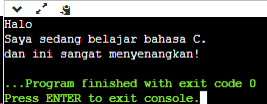
\includegraphics[width=0.5\linewidth]{../P1/img/screenshot0006.png}
	\caption{}
	\label{fig:screenshot0006}
\end{figure}

\item[Contoh \thesubsection.7] Menggunakan escape sequence \verb*|\t| mengubah tab.
\begin{lstlisting}[language=c]
#include <stdio.h>
int main(void)
{
	printf("Nama \t\t: Rahmad Rahardi\n");
	printf("Alamat \t\t: Bendungan Hilir Jakarta\n");
	printf("Tempat Lahir \t: Jakarta\n");
	printf("Tanggal Lahir \t: 30 Pebruari 2000\n");
	
	return (0);
}
\end{lstlisting}
\begin{figure}[H]
	\centering
	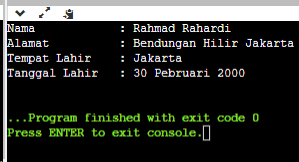
\includegraphics[width=0.5\linewidth]{../P1/img/screenshot0007.png}
	\caption{}
	\label{fig:screenshot0007}
\end{figure}
\end{description}

\subsection{Tugas Pendahuluan}
\begin{enumerate}
	\item Cobalah buat suatu program yang dapat menerima input berupa nama dan NRP kemudian menampilkannya pada layar.
	\item Buat program yang meminta pengguna memasukkan suhu dalam Celsius dan kemudian mengonversinya ke Fahrenheit.
\end{enumerate}

\begin{center}
    \colorbox{cyan!30}{\parbox{0.8\linewidth}{\textbf{Opsional:} Pelajari Git dan Github. Anda dapat memulai pembelajaran dari sumber berikut ini: \\ \href{https://github.com}{GitHub - https://github.com} \\ \href{https://git-scm.com/doc}{Git -https://git-scm.com/doc}}}
\end{center}